\RequirePackage{fixltx2e}
%\documentclass[superscriptaddress,showkeys, nofootinbib, pre, aps,twocolumn]{revtex4-1}
\documentclass[superscriptaddress,showkeys, nofootinbib, pre, aps]{revtex4-1}

% PRL look and style (easy on the eyes)
% Two-column style (for submission/review/editing)
%With revtex4, the prb class option places all ancillary maketitle info in footnotes with the bibliography FYI

\usepackage[english]{babel}
\usepackage{amsmath,amsthm}
\usepackage{amsfonts}
\usepackage{latexsym}
\usepackage{color}
\usepackage{graphicx}
\usepackage{amssymb}
\usepackage{dcolumn}
\usepackage{boxedminipage}
\usepackage{soul}
%\usepackage{longtable}
\usepackage{verbatim}
\usepackage{caption}
%\usepackage{caption}
%\usepackage[version=3]{mhchem}
\usepackage{booktabs}
\usepackage{multirow}
\usepackage{float}
\usepackage{subcaption}
\usepackage{fancyhdr}
%\usepackage[margin=1.0in]{geometry}
%\usepackage{titling}
\usepackage[small]{titlesec}
%\usepackage{natbib}
\usepackage{palatino}
%\usepackage{mathpazo} %Palatino math fonts -- meh, not as good as I thought it might look
\usepackage[colorlinks=true,citecolor=blue,linkcolor=blue]{hyperref}
\renewcommand{\arraystretch}{1.2} %(or 1.3) -- More space between table rows
\newcommand{\ra}[1]{\renewcommand{\arraystretch}{#1}}
%Remove space to the vertical edges:
%\begin{tabular}{@{}lll@{}}

%\newcommand{\bfm}[1]{{\bf #1}}              % proper boldface for math environment
\newcommand{\bfm}[1]{{\mbox{\boldmath{$#1$}}}}
%\newcommand{\bfm}[1]{{\bf #1}}
\newcommand{\expect}[1]{\left \langle #1 \right \rangle}                % <.> for denoting expectations over realizations of an experiment or thermal averages
\newcommand{\x}{\bfm{x}}
\newcommand{\y}{\bfm{y}}
\newcommand{\f}{\bfm{f}}
\newcommand{\bfc}{\bfm{c}}
\newcommand{\hatf}{\hat{f}}

\newcommand{\bTheta}{\bfm{\Theta}}
\newcommand{\btheta}{\bfm{\theta}}
\newcommand{\bhatf}{\bfm{\hat{f}}}
\newcommand{\Cov}[1] {\mathrm{Cov}\left( #1 \right)}
\newcommand{\Ept}[1] {{\mathrm E}\left[ #1 \right]}
\newcommand{\Eptk}[2] {{\mathrm E}\left[ #2 \,|\, #1\right]}
\newcommand{\T}{\mathrm{T}}                                % T used in matrix transpose
\newcommand{\Ww}[1] {{\mathrm w}\left( #1 \right)}
\newcommand{\Ht}{\bfm{\tilde{H}}}
\newcommand{\gt}{\bfm{\tilde{g}}}
\newcommand{\Dt}{\bfm{\tilde{D}}}
\newcommand{\pt}{\bfm{\tilde{p}}}
\newcommand{\Nt}{\bfm{\tilde{N}}}
\newcommand{\ft}{\bfm{\tilde{f}}}
\newcommand{\dhdl}[1]{\left.\frac{\partial H}{\partial \lambda}\right|_{\lambda=\lambda_{#1}}}
\newcommand{\dudl}[1]{\left.\frac{\partial u}{\partial \lambda}\right|_{\lambda=\lambda_{#1}}}
\newcommand{\ro}[1]{r_{#1}^{\mathrm{old}}}
\newcommand{\rn}[1]{r_{#1}^{\mathrm{new}}}

\DeclareSymbolFont{AMSb}{U}{msb}{m}{n}
\DeclareMathSymbol{\N}{\mathbin}{AMSb}{"4E}
\DeclareMathSymbol{\Z}{\mathbin}{AMSb}{"5A}
\DeclareMathSymbol{\R}{\mathbin}{AMSb}{"52}
\DeclareMathSymbol{\Q}{\mathbin}{AMSb}{"51}
\DeclareMathSymbol{\I}{\mathbin}{AMSb}{"49}
\DeclareMathSymbol{\C}{\mathbin}{AMSb}{"43}


% ----------------------------------------------------------------  Begin Document --------------
\begin{document}
%\setlength{\droptitle}{-80pt}
\title{A review of adaptive determination of free energies in expanded ensemble simulations}%

\author{Arjan C. Kool}
\affiliation{Department of Chemical Engineering, University of Virginia, Charlottesville, Virginia 22904-4741, United States}

\author{Michael R. Shirts\thanks{Corresponding author.  Electronic address: michael.shirts@virginia.edu}}%
\email{michael.shirts@colorado.edu}
\affiliation{Department of Chemical and Biological Engineering, University of Colorado, Boulder, CO 80309, United States}
%\email{}


\date{\today}%
%\pagestyle{empty}
% ----------------------------------------------------------------Abstract----------------------
\begin{abstract}

A review on the theory of the different Monte Carlo expanded ensemble algorithms such as Wang-Landau, Accelerated Weighted Histogram, the transition matrix approach, Self-Adjusted Mixture Sampling, and other modifications.
\end{abstract}
%\keywords{Computational Methods, Expanded Ensemble, Importance Weights, Molecular Simulation, Monte-Carlo, Multistate Bennett acceptance ratio, Nanotechnology, Thermodynamics, Wang-Landau}
\maketitle
%------------------------------------------------------------------------ End Title ----------------
\begin{comment}
Just in case, e.g:

\begin{widetext}
long equation goes here
\end{widetext}
\end{comment}
%----------------------------------------------------------------------- Introduction--------------
\section{\label{sec:intro}Introduction}
%{\bf Explain the problem in more detail. Answer the why? in more depth.}

%For complex molecules, simple equations of state are insufficient to give reliable thermodynamic properties and full molecular simulations are the best way to predict thermodynamic properties.  

In Monte Carlo (MC) and molecular dynamics (MD) simulations, equilibrium thermodynamic properties
are computed for a given molecular system as averages over the
configuration of the system for a single thermodynamic state. However,
conventional MC or MD methods will not work to sample most interesting molecular systems sufficiently, ranging from spin glasses to polymers to proteins, because the simulation gets stuck in metastable free energy minima. Computing properties of such systems over large numbers of thermodynamic states or conditions therefore becomes extremely expensive or effectively impossible.

%If there are $N$ possible parameters for a system and 10 possible choices for each parameter, then there $10^{N}$ total ensembles that must be simulated.  The problem is thus combinatorially large, and it is impossible to directly perform $10^{N}$ separate statistical sampling simulations.  This problem has important efficiency implications for computational chemical design using MC methods.

Expanded or generalized ensemble methods are a broad class of methods designed to help overcome sampling difficulties. Expanded ensemble algorithms involve joint random walks in configuration space $\vec{x}$ and some auxiliary variables $\vec{\lambda}$~\cite{shirts_gibbssamp}.  These auxiliary variables are chosen such that they affect the probability of each state, usually by modifying the Hamiltonian.  We note these $\vec{\lambda}$ are not collective variables, i.e. functions of the coordinates. These methods which accelerate sampling in collective variables are a separate set of methods that are extremely useful, and share some of the same features and variants, but we will not cover them here.

Sampling in these auxiliary variables can improve the configuration sampling if rates of transition between configurational states are lower at some value of the auxiliary variables. For example, if a ligand is bound to a receptor in a long-lasting metastable state, one can add the auxiliary variable of the coupling of the ligand to the receptor, such that at $\lambda=0$ the system is the fully physical system, and $\lambda=1$ the ligand is decoupled from the system.  If one performs expanded ensemble sampling with this $\lambda$, then when the ligand is less coupled to the environment, it will be able to unbind and rebind in lower free energy configurational ensemble. If the kinetic barriers are sufficiently high in the unmodified system, and are lowered sufficiently in the system with auxiliary variables, then the expanded ensemble system will be able to sample the important configurations in the expanded ensemble simulation despite the additional work required to sample the $K$ subensembles.  If the barriers are lowered linearly in $K$ by performing expanded ensemble simulation with $K$ subensembles, then this simulation will increase the rate of sampling exponentially. This should be recognized as a bit of a handwaving argument, as rarely do the auxiliary variables ONLY decrease barriers; they also change the probabilities of the states sampled, making speedup arguments somewhat complicated. But it gives a sense of what may be possible.

A large variety of auxiliary variables are possible, as such variables can be literally anything that affect the probability of the states. Besides decoupling one part of the system from the rest of the system, other possible auxiliary variables could include those defining a series of biasing potentials that restrain the system in some way, which allows the system to be passed back and forth between the restrained systems. They also could include external thermodynamic variables including the temperature (a variant called simulated tempering), pressure, and chemical potential.  The "right" choice of auxiliary variable to accomplish a given type of improve sampling is beyond the scope of this review; we will deal only with questions of creating simulations that can visit all the states defined.

Each choice of the auxiliary variables results in a subensmble within an \emph{expanded}
ensemble.  Transitions between the subensembles, each of which can be labeled by $\vec{\lambda}$, can is most generally performed by MC or MD. In theory, one can perform dynamics in a continuous $\vec{\lambda}$ space as well~\cite{lambda_dynamics}, but that introduces additional complications we will not address in this review, so we will assume that the transitions between subensembles are performed by some variety of MC.

Simply introducing motion in an auxiliary variable does not alone solve the sampling problem alone. If we sample in the joint $(x,\lambda)$ space, without any modifications of the relative probability of the separate subensembles labeled by $\lambda$, we would soon find that we would be spending more time with values of $\vec{\lambda}$ in states with lower free energies. In fact, the time we spend in each subensemble is proportional to total integrated probability over the entire $x$ set, which is just the partition function of the subensemble $Z(\vec{\lambda}) = \int e^{-u(\vec{x},\vec{\lambda})} d\vec{x}$. If we wish to visit lower probability states, we need to add to our MC algorithm for transitioning between subensembles some additional biasing potential $g(\vec{\lambda})$. Note that it its only a function of $\vec{\lambda}$, not $x$.  

So what should we choose $g_k$ to be for each state? This is perhaps the single most important and complicated issue in the expanded ensemble framework, second perhaps only to the choice of the auxiliary variable itself. If the probability of visiting a state is $Z(\vec{\lambda})$ as noted above, then in order to visit all of the states equally (which is a natural choice, though others choices may be possible) we could bias each state by $1/Z(\vec{\lambda})$, one over the partition function. Even if we wanted something a bit different than equal distribution of states, for example, if we wanted to spend more time at states with the lowest kinetic barriers for important configurational transitions, we would still need the weights to be relatively close to $1/Z_k$, because otherwise we would not spend very much time at most $k$. 

Of course, the goal of our simulations themselves is often to calculate free energy differences between states, or equivalently the partition functions, so it all becomes somewhat circular; we need to know the partition function to calculate the partition function. Thus, we will need some sort of adaptive method that allows us to gradually learn the partition function of all of the subensembles as the simulation progresses and spend time at each state.

Generally, such algorithms to learn $g_k$ adaptively are classified as ``visited states'' algorithms, because we collect statistics about the states as we visit them, and then update our $g(\vec(\lambda))$. Consider the free energies of the physical states as being represented holes/wells of some initially unknown depth proportional to their probability.  A
fictitious random walker visits the different states labeled by $\vec{\lambda}$ as the simulation proceeds, dropping ``dirt'' into the
wells, thus gradually building up the importance weights.  At the end
of the simulation, when all states are visited equally, one counts how
much much ``dirt'' the walker has added to each state's weight to
achieve equal sampling. The negative logarithm of this accumulated dirt simply is the free energy of the state (normalized by the temperature).  This analogy is illustrated in
Figure~\ref{fig:EXEanalogy}.

\begin{figure}[H]
        \centering
        \begin{subfigure}[b]{0.3\textwidth}
                \centering
                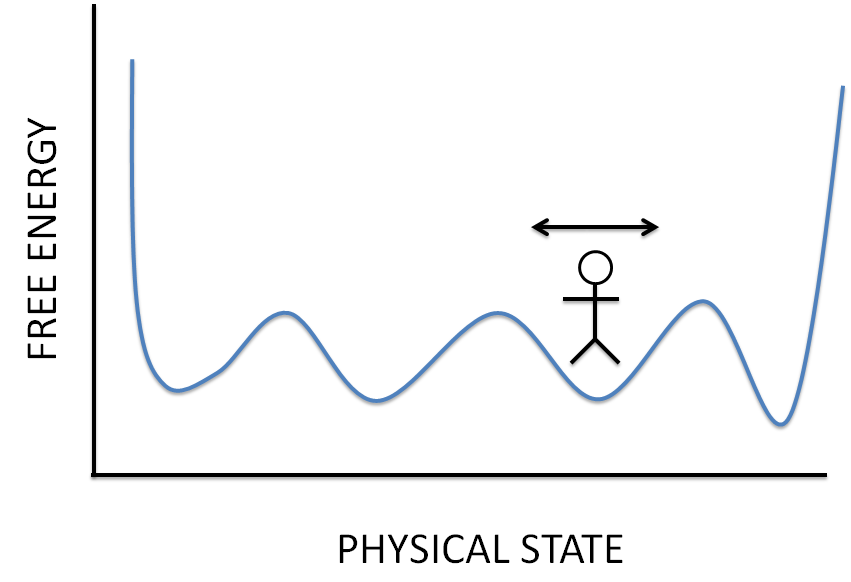
\includegraphics[width=\textwidth]{figures/emptywell.png}
                \caption{Beginning of Simulation}
                \label{fig:emptywell}
        \end{subfigure}%
        ~ %add desired spacing between images, e. g. ~, \quad, \qquad etc.
          %(or a blank line to force the subfigure onto a new line)
        \begin{subfigure}[b]{0.3\textwidth}
                \centering
                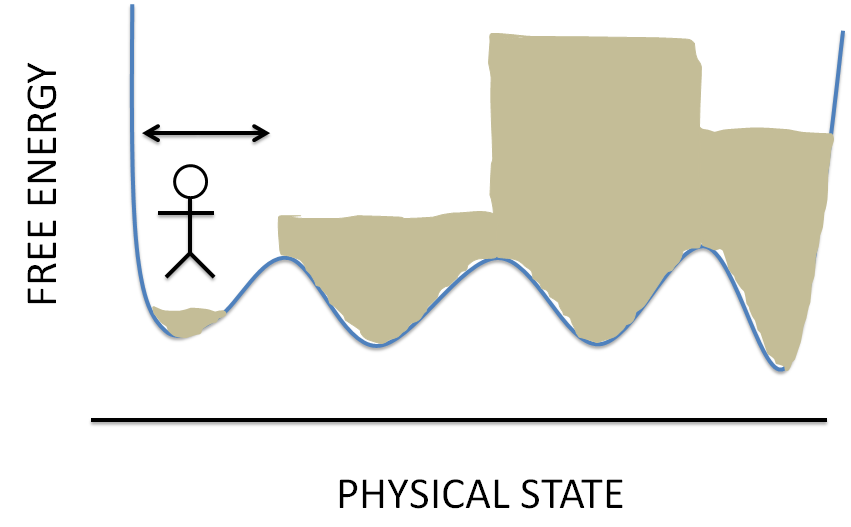
\includegraphics[width=\textwidth]{figures/halfwell.png}
                \caption{During Simulation}
                \label{fig:halfwell}
        \end{subfigure}
        ~ %add desired spacing between images, e. g. ~, \quad, \qquad etc.
          %(or a blank line to force the subfigure onto a new line)
        \begin{subfigure}[b]{0.3\textwidth}
                \centering
                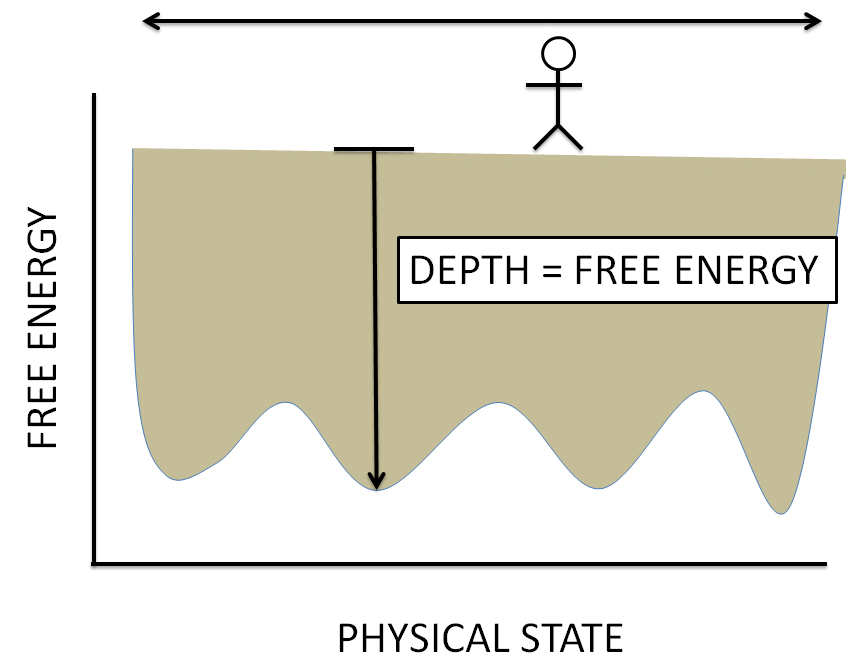
\includegraphics[width=\textwidth]{figures/fullwell.png}
                \caption{End of Simulation}
                \label{fig:fullwell}
        \end{subfigure}
        \caption{The expanded ensemble hole analogy. (\ref{fig:emptywell}) At the beginning the weights are unknown. (\ref{fig:halfwell}) As the simulation proceeds, a random walker samples the states and deposits ``dirt'' in each well.  The short arrow over the random walker signifies uneven sampling of the states.  (\ref{fig:fullwell}) At the end of the simulation, the weights become the free energies given by the height of ``dirt'' in each well.  The random walker now samples all states equally, as illustrated by the long bar over the walker which now extends over all of state space} \label{fig:EXEanalogy}.
\end{figure}

The original visited states algorithm used in original expanded ensemble simulations was typically the Wang-Landau algorithm, in which one state's weight is updated only at time it is is visited during the random walk in state space.
\cite{wang-landau:prl:2001:wang-landau}.  Several algorithmic modifications to the original Wang-Landau algorithm have been proposed
and there have been multiple studies of the convergence and saturation of error of the original algorithm and its
variants~\cite{Belardinelli2007, Belardinelli2008}, which we will discuss in more detail below. For example, because we can compute the Boltzmann weight of neighboring values of $\vec{\lambda}$, it is possible to do better than the simplest Wang-Landau algorithm. First, to examine the possibilities of improved multistate adaptive methods, it is instructive to start with the theoretical basics, and examine the building blocks of the methods for calculating free energies in an adaptive manner.

%Multistate reweighting methods such as the Multistate Bennet
%acceptance ratio (MBAR) involve gathering statistical information
%determined by one set of molecular parameters using data from another
%set of molecular parameters \cite{shirts-chodera:jcp:2008:mbar}.
%Algorithms incorporating multistate reweighting into an EXE scheme,
%such as the recently proposed Accelerated Weight Histogram method,
%should enhance importance weight estimation because they incorporate
%data from nearby thermodynamic states, not just the sampled one.

%Chemical design situations such as drug and heteropolymer design require simulating and sampling large numbers, thousands to millions of different thermodynamic states.  For example, in drug design, the free energy of binding in the protein-ligand system must be minimized for a exceedingly large number of potential ligands.  In this study, we seek to propose a new EXE algorithm, derived from MBAR, to help converge free enregies faster in EXE simulations.  

%------------------------------------------------------------------- Theory----------------------
\section{\label{sec:theory}Theory}
%\textbf{Use this section to introduce the concepts of Expanded Ensembles using WL and WWL.  Also address the criteria for state transitions: Metropolis(just two nearest neighbors version), Gibbs Sampling and Metropolized Gibbs -- Introduce MBAR too}.
%Before describing our suggested algorithmic modifications
%(\emph{Weighted Wang-Landau method}, Section~\ref{sec:wwl}).

We first review in more detail existing theoretical approaches to moving between states calculating free energies of states. Again, we will generally restrict ourselves to the case where there are only $K$ discrete values of $\vec{\lambda}$ that are of interest, leaving "$lambda$-dynamics" approaches out of the scope for now.

\subsection{\label{sec:ensembles}Thermodynamic states and thermodynamic ensembles}

To be as general as possible, we describe the expanded ensemble and replica exchange algorithms as sampling a mixture of $K$ thermodynamic
states.  Here, a \emph{thermodynamic state} is parameterized by a vector of time-independent thermodynamic parameters $\lambda$.  For
notational convenience and to make what follows general, we define the
\emph{reduced potential}~\cite{shirts-chodera:jcp:2008:mbar} $u(x)$ of
a physical system,
\begin{eqnarray}
u(x) &=& \beta \left[ \mathcal{H}(x) + p V(x) + \sum_i\mu_i n_i(x) + \cdots \right], \label{equation:reduced-potential}
\end{eqnarray}
corresponding to its thermodynamic state, where $x$ denotes the
configuration of the system specifying any physical variables allowed
to change, including the volume $V(x)$ (in the case of a constant
pressure ensemble) and $n_i(x)$ the number of molecules of each of
$i=1,\ldots,M$ components of the system, in the case of a (semi)grand
ensemble.

The reduced potential is a function of the Hamiltonian $\mathcal{H}$, the
inverse temperature $\beta = (k_B T)^{-1}$, the pressure $p$, and the
vector of chemical potentials for each of $M$ components $\mu_i$.
Other thermodynamic parameters and their conjugate coordinates can be
included in a similar manner, or some of these can be omitted, as
required by the physics of the system.  We denote the set of all
thermodynamic parameters by $\lambda \equiv \{\beta, \mathcal{H}, p, \vec{\mu},
\ldots\}$. We will assume that the configuration space for each choice of $\vec{\lambda}$ has the same size, so different Hamiltonians do not directly change the phase space, but the Boltzmann weights of a given $x$ can vary significantly between choices of $\vec{\lambda}$. This does provide some restriction; for example, it rules out the introduction/elimination particles as function of $\lambda$, or disappearing/appearing hard spheres.

We next denote a configuration of the molecular system by $x \in
\Gamma$, where $\Gamma$ is allowed configuration space, which may be
continuous or discrete.  A choice of thermodynamic state gives rise to
set of configurations of the system that are sampled by a given
time-independent probability distribution at equilibrium.  So each $x$
will have associated unnormalized probability density $q(x)$, which is
a function of $\lambda$, where $q(x) > 0$ for all $x \in \Gamma$. If
we define the normalization constant, or \emph{partition function},
$Z$ as:
\begin{eqnarray}
Z &\equiv& \int_\Gamma dx \, q(x)
\end{eqnarray}
we can define a normalized probability density
\begin{eqnarray}
\pi(x) &=& Z^{-1} \, q(x).
\end{eqnarray}

A physical system in equilibrium with its environment obeying
classical statistical mechanics will sample configurations distributed
according to the Boltzmann distribution,
\begin{eqnarray}
q(x) &\equiv& e^{-u(x)} .
\end{eqnarray}

In this review, we consider a set of $K$ thermodynamic states defined
by their thermodynamic parameter vectors, $a_k \equiv \{\beta_k,
\mathcal{H}_k, p_k, \vec{\mu}_k, \ldots\}$, with $k = 1,\ldots,K$, where $H_k$
denotes any modifications of the Hamiltonian $H$ as a function of $k$,
including biasing potentials.  Each new choice of $k$ gives rise to a
reduced potential $u_k$, unnormalized and normalized probability
distributions $q_k(x)$ and $\pi(x,k)$, and a partition function $Z_k$.
To ensure that any configuration $x$ has finite, nonzero density in
all $K$ thermodynamic states, we additionally require that the same
thermodynamic parameters be defined for all thermodynamic states,
though their values may differ at different states.

We note that frequently in the development of methods,
there is an assumption that the states contain some
natural ordering. In other words, that the configurations that result
from simulations at $i$ are more similar to the configurations
generated in state $i-1$ and $i+1$ than to any other states.  A number
of methods assume this ordering, which may not exist in the general
case.  When states are selected points along a single variable
$\lambda$, such an ordering can generally be defined, though there is no guarantee that they WILL be ordered. When states are selected in a
multidimensional state space parameterized by a vector $\lambda$, no such ordering may exist, and some of the methods may break down, or need some sort of adaptation.

\begin{comment}
\begin{itemize}
\item Canonical
\item Expanded -- paper: \cite{lyubartsev:jcp:1992:expanded-ensembles}
\item Acceptance Criteria \begin{itemize}\item Metropolis
\item Gibbs
\item Metropolized Gibbs\end{itemize}
\item MBAR - provably minimum variance free energy estimator; will serve as our control/true state for all simulations \cite{shirts-chodera:jcp:2008:mbar}.
\end{itemize}
\end{comment}

\subsection{Expanded Ensembles \label{sec:expandedensembles}}

In an expanded ensemble simulation~\cite{lyubartsev:jcp:1992:expanded-ensembles}, a single replica or ``walker'' (because it walks between states) samples pairs of coordinates $(x,k)$ from a joint distribution of configurations $x \in \Gamma$ and state indices $k \in \{1,\ldots,K\}$ given by,
\begin{eqnarray}
\pi(x,k) &\propto& \exp[-u_k(x) + g_k] ,
\end{eqnarray}
where $g_k$ is an state-dependent weighting factor.
This space is therefore a {\em mixed}, {\em generalized}, or {\em expanded} ensemble which samples from multiple thermodynamic sub-ensembles (each defined by $\lambda$) simultaneously.
$g_k$ is chosen to give a specific weighting of each sub-ensemble in the expanded ensemble, and is generally determined
through some iterative procedure~\cite{lyubartsev:jcp:1992:expanded-ensembles,marinari-parisi:europhys-lett:1992:simulated-tempering,wang-landau:prl:2001:wang-landau,park-ensign-pande:pre:2006:bayesian-weight-update,park-pande:pre:2007:choosing-weights-simulated-tempering,li-fajer-yang:jcp:2007:simulated-scaling,chelli:jctc:2010:optimal-weights-expanded-ensembles}, the various choices of which we will explore.
The set of $g_k$ is frequently chosen to give each thermodynamic ensemble equal probability (so-called ``perfect weights''~\cite{park-pande:pre:2007:choosing-weights-simulated-tempering}), in which case $g_k=-\ln Z_k$, but they can be set to arbitrary values in order to obtain any desired relative frequency of each of the subensembles.

In the context of Gibbs sampling, an expanded ensemble simulation proceeds by alternating between sampling from the two conditional distributions,
\begin{eqnarray}
\pi(x | k) &=& \frac{q_k(x)}{\int_\Gamma dx \, q_k(x)} = \frac{e^{-u_k(x)}}{\int_\Gamma dx \, e^{-u_k(x)}} \\
\pi(k | x) &=& \frac{e^{g_k}q_k(x)}{\sum\limits_{k'=1}^K e^{g_{k'}}q_{k'}(x)} = \frac{e^{g_k - u_k(x)}}{\sum\limits_{k'=1}^K e^{g_{k'} - u_{k'}(x)}} .\label{equation:expanded-ensemble-gibbs-update}
\end{eqnarray}

In all but trivial cases, sampling from the conditional distribution $\pi(x | k)$ must be done using some form of Markov chain Monte Carlo sampler that generates correlated samples (we consider MD here a subset of Markov chain MC approaches), due to the complex form of $u_k(x)$ and the difficulty of computing the normalizing constant in
the denominator~\cite{jun-s-liu:mcmc}. Typically, Metropolis-Hastings
Monte Carlo~\cite{metropolis:jcp:1953:metropolis-monte-carlo,hastings:biometrika:1970:metropolis-hastings}
or molecular dynamics is used~\cite{footnote3}, generating an updated
configuration $x^{(n+1)}$ that is correlated with the previous
configuration $x^{(n)}$.  Although complicated, this is the fundamental problem in molecular simulation, so many efforts have been made to efficiently solve this problem.  We'll assume for now that we are doing some variety of straightforward configurational sampling, and not more advanced sampling methods that modify the configurational probability distribution. It is possible to combine these techniques with expanded expanded ensemble techniques, where accelerated sampling with different parameters is carried out at each separate ensemble member, but such approaches are beyond the scope of this review.

The sampling in $\pi(k|x)$ is generally much simpler than sampling in $\pi(x|k) $, since there are only $k$ states to choose from rather than an extremely complicated configurational space if $x$.  If we have a set of  discrete states which can be enumerated, we can simply calculate $u_k(x)$ for each state and select randomly with $\pi(k|x)$, which is Gibbs sampling~\cite{chodera:jcp:2011}. The probabilities of transition only depend on the reduced energy differences $\Delta u_{ik}(x) = u_i(x) - u_k(x)$, which is often much cheaper to calculate than $u_k(x)$ is, as it usually only involves the part of the system that depends on the auxiliary variables.

Other Monte Carlo methods can of course be used to sample between states.  One can perform Metropolis-Hastings sampling between the current state $i$ and some other state $j$. This works much more efficiently if one can identify which states are neighbors to $i$, i.e. have high overlap compared to to other states. This works especially well in one dimension if a natural ordering exists---neighboring temperatures, for example, or neighboring states along the pathway of disappearance of a molecule. Then one can simply perform Metropolis-Hasting moves between neighbors $i-1$ and $i+1$ with, 50/50 probability.  This is generally the most common way that expanded ensemble dynamics in state spaces is implemented, as it only involves calculating the energy at two neighboring states. One can also "metropolize" Gibbs sampling itself, introducing acceptance and rejection step in a way that can be shown to always improve the probability of moving from the current state~\cite{chodera:jcp:2011} though sometimes not by very much. The various ways to move between states have been relatively well-explored~\cite{chodera:jcp:2011}, so we will not explore them further in this review. If dealing with a 1-dimensional array of states, all choices of state dynamics should work fine.

And the above covers virtually all of the theory of expanded ensembles---except, of course, \emph{how} to choose an auxiliary variable $\lambda$, which we will not cover, in this review, and the choice of $g_k$ that gives rise to desired behavior, which will be the main topic of discussion of the rest of this review.

\subsection{\label{sec:equilibrium_methods}Equilibrium Methods}

We will first assume that we are carrying out an expanded ensemble simulation with the weights $g_k$ fixed during the simulation. This may seem odd, since the whole idea is that we want to iteratively guess the right $g_k$.  Although we do require some guess of $g_k$ to start with, all the methods work for any $g_k$, with caveats discussed below, even if the $g_k$ are not exactly the ones giving the desired probability distribution. Therefore, one can run until the $g_k$ are \emph{approximately} correct (i.e. give the roughly desired distribution of states) using some other approach, run for some amount of time with fixed weights, and use the methods above.  

The one caveat is that if we have approximate $g_k$, then we will could have widely varying numbers of samples at each of the $k$ states. If there are too few samples at some states, then it may not be possible to calculate all of the free energy differences accurately---and if there are \emph{no} samples at some states, it may not be possible to calculate free energy differences involving those states at all.   

If the $g_k$ are fixed, then the overall behavior of the simulations is pretty much like any set of simulations that generate configurations from $k$ separate states, either $k$ independent simulations, or using methods such as replica exchange.  This may not be ideally efficient, as significant time may be taken to generate approximate $g_k$ that is not efficiently used, but does have the advantage of being simple---once we have samples collected with fixed $g_k$, we can use straightforward data analysis techniques for equilibrium samples. Of course, unlike replica exchange, there is only one simulation which contains all the states, and for many analysis methods, the output files must be parsed appropriately to separate all samples based on which states they are sampled from.  

We will express the following in terms of finding $\Delta f_{ij}$ between two states, but of course once we have the free energy difference between the states, this is the same as finding the difference in weights $g_{ij}$ between two states. If we have estimates of the differences $g_{ij}$, we can estimate the weights $g_k$.  It may be that the matrix of $g_{ij}$ is inconsistent, since there are $\frac{K(K-1)}{2}$ differences, but only $K-1$ independent $g_k$ ($K-1$ since the $g_k$ are only defined up to an additive constant). For all methods except MBAR below, it is best to set on $g_1 = 0$ and just take neighboring states in pairs; this will uniquely define the $g_k$. For MBAR, one can show that the $g_{ij}$ obtained are consistent with a single set of $g_k$.

\subsubsection{Directly measured ratios}

The free energy difference between state $i$ and state $j$ $f_{ij}$ can be estimated as:
\[
\Delta f_{ij} = -(\ln N_j/N_i) + (g_{i}-g_{j})
\]
Where $N_i$ and $N_j$ are the numbers of samples collected between 
In practice, this ends up being fairly hard to calculate accurately between states that far are widely spaced, as if the fixed weights $g_k$ are poor, then some states will have very few samples. It is best to calculate this estimate from states that are relatively close to each other (for example, $j = i+1$ if the $K$ states happen to be ordered), and then chain together estimates from neighboring states to span the entire range of
$K$. 
The uncertainty in this ratio can be calculated by treating the $N_i$ as a multinomial Bernoulli distribution.  The variance in $\langle N_i\rangle$ is $(N_i)(1-N_i/N)$, and the covariance between $N_i$ and $N_j$ is $-N_iN_j/N$. The uncertainty formula for ratios is therefore:
\begin{eqnarray}
\sigma^2(A/B) &=& (A/B)^2\left[\frac{\sigma_A^2}{A^2} + \frac{\sigma_B^2}{B^2}-2\frac{\sigma_{AB}}{AB}\right] \\
 \sigma^2(N_j/N_i)&=& \left(\frac{N_j}{N_i}\right)^2\left[ \left(\frac{1}{N_j}-\frac{1}{N}+\frac{1}{N_i}-\frac{1}{N}\right)+\frac{2}{N}\right] \\
&=& \left(\frac{N_j}{N_i}
\right)^2\left(\frac{1}{N_j}+\frac{1}{N_i}\right)
\end{eqnarray}
The error in the logarithm of the ratio is then:
\begin{equation}
\sigma(-\ln(N_j/N_i)) = \frac{\sigma(N_j/N_i)}{\frac{N_j}{N_i}}  = \sqrt{\frac{1}{N_j}+\frac{1}{N_i}}
\end{equation}
which scales properly with $\sqrt{N}$ samples taken.
\subsubsection{Thermodynamic Integration (TI)}
If we can compute the change in the potential as a function of the coupling constant for the state, then $\Delta f_{ij}$ can be estimated as:
\[
\Delta f_{ij} = -\frac{\Delta \lambda_{ij}}{2}\left[\left\langle \dudl{i} \rangle_i + \langle \dudl{j} \right\rangle_j \right]
\]
Clearly, this is only simple to apply if one imposes a single coupling parameter $\lambda$ connecting the states. In practice, it makes the
most sense to compute this only between states that are next to each
other ($i$ and $i+1$), as the numerical integration has the least
approximation over a short range. The total free energy of state $k$
will again be the sum over all states $i<k$.  Note that this integral
does not include the weights $g_i$ and $g_j$; it's a bit subtle, but
the derivatives are the same regardless of what the weight values are,
as the sub-ensemble stays the same. Error estimates are readily available. We will generally not consider TI this further in the case of discrete states, though it will become more useful in the case of continuously varying states (though it's only occasionally used even there).

\subsubsection{Exponential averaging}
If we have fixed weights, and carry out expanded ensemble simulations, then the total free energy difference between any two states can be estimated as:
\[
\Delta f_{ij} = -\ln \frac{1}{N_i}\sum_{n=1}^{N_i} e^{-\Delta u_{ij}(x_n)}
\]
where $\Delta u_{ij} = u_j - u_i$, and the $N_i$ samples are from the $i$th state.  We can also write this more compactly as:
\[
\Delta f_{ij} = -\ln \langle e^{-\Delta u_{ij}}\rangle_i
\]. 
This is sometimes referred to as the Zwanzig relationship, and error estimates are again readily available. One can apply this to calculate the free energy differences, and therefore estimate the $g_k$.

\subsubsection{Bennett Acceptance Ratio}

The Bennett acceptance ratio method is the lowest variance reweighting method to calculate free energy differences between two states using data from two states.  There are a large number of ways to write out the method~\cite{bennett:jcp:1976:fe-estimate,shirts_comparison_2005,fenwick-escobedo:jcp:2003:replica-exchange-expanded-ensembles}.
The form we choose to use here, write the
free energy difference $\Delta f_{ij} = f_j-f_i$ and $\Delta u_{ij}(x)
= u_j(x)-u_i(x)$, and set $M = \ln N_j/N_i$ to get:
\begin{eqnarray}
e^{\Delta f_{ij}} &=& e^{c+M}\frac{\left \langle \left[1 + e^{M + c - \Delta u_{ij}(x)}\right]^{-1}\right \rangle_j}
  {\left \langle \left[1 + e^{-M - c + \Delta u_{ij}(x)}\right]^{-1}\right \rangle_i}
\end{eqnarray}
The lowest variance estimate of free energy is obtained when $c=\Delta
f_{ij}$, requiring a solution of a self-consistent set of equations. It is an asymptotically unbiased estimator for any choice
of $c$.  So in the case of fixed $c$, this is not an iterative
equation.  Bennett and others~\cite{fenwick-escobedo:jcp:2003:replica-exchange-expanded-ensembles,Paliwal_comparison_2011} have
shown that when $c_k$ is relatively close to $f_k$ (within 1--2 $k_B T$)
it is still an excellent estimate of the free energy.  Thus, one can
maintain the averages in the numerator and the denominator for a range
of possible $c_k$, and whichever gives the free energy closest to
$c_k$, that answer is used, essentially precalculating the
self-consistent iteration.  Again, if we are looking for the optimal value,
then we will need to solve the equation self-consistently, which can
be done straightforwardly by a number of methods, but in many cases, it may not be necessary to do this iteration step, trading multiple repetitions of the solution but avoiding iteration.

\subsubsection{Multistate Bennett Acceptance Ratio}
If we have fixed weights, and carry out expanded ensemble simulations, then the total free energy difference between any two states will simply be:
\[
f_i = -\ln \left[\sum_{n=1}^N \frac{\exp(-u_i(x_n))}{\sum_k N_k \exp(f_k-u_k(x_n))}\right]
\label{eq:MBAR}
\]
$\Delta f_{ij}$ can be computed directly from the $f_i$.  MBAR allows the computation of asymptotically correct uncertainties in the $\Delta
f_{ij}$'s, as it can take into account the correlations in $f_i$ and $f_j$ due to them being estimated from the same set of data.

As in the case of BAR, we can construct asymptotically unbiased
estimators for MBAR that are not self-consistent, functions of constants $c_k$ that give correct free energy estimates, and which
converge to the MBAR estimate when the input $c_k=f_k$.  For example, we can use:
\[
f_i = -\ln \left[\sum_{n=1}^N \frac{\exp(-u_i(x_n))}{\sum_k N_k \exp(c_k-u_k(x_n))}\right]
\label{eq:unoptimizedMBAR}
\]
Which clearly converges to MBAR in the case that $c_k=f_k$, and can be
shown using the methods of Ref.~\cite{shirts-chodera:jcp:2008:mbar} to be a valid
estimator of the free energy~\footnote{To derive from MBAR, take
  $\alpha_{ij}(x)=\frac{N_j e^{f_i}}{\sum_{k=1}^K N_k
    e^{c_i-u_i(x)}}$}. The properties of this estimator have not been
explored extensively, though anecdotally, it is harder to work with a the non-iterative variant MBAR
than the non-iterative BAR variant, as one needs ALL $c_k$ to be close
to $f_k$, which is a more difficult condition than having only one
$c_k$ close to a single $f_k$. This method is generally not used for equilibrium simulations for this reason.
 
\subsection{\label{sec:equilibrium_methods}Equilibrium Methods using the last $N$ states}

In theory, one could start a simulation, and then calculate the free energies of the $k$ states that have samples up to that point, and use these free energies as estimates of the $g_k$, and repeat, using either the sampled states since the beginning of the simulation, or just the last $N$ sampled states.
If using the formulas above, then the amount of time it takes to compute a free energy will depend on the number of samples $N$, which, as the simulation proceeds, will take longer and longer.  For some methods, this may involve negligible time, but for others, especially those that involve solving nonlinear equations at each step like MBAR, this could be time-limiting.

Can we therefore carry out a computation of the $f_k^N$ using only the last $N_I$ data points, and an estimate of the free energy at $f_k^{N-N_I}$.  How much accuracy does this lose versus calculating the free energy at every state? As we small see, any method which does not involve a solving a system of equations can express $f_k^{N+N_I}$ exactly as a function of $f_k^{N}$ (or possibly a small number of other statistics computed over the first $N$ points) and the last $N_I$ data points collected.

For compactness, we write $N_i^{N+N_I} - N_i^{N} = \delta N_i$ $\delta f_i = f_i^{N+N_I} - f_i^{N}$, and $\delta \Delta f_{ij} =\Delta f_{ij}^{N+N_I} - f_{ij}^{N}$. Note that the first two are vectors, and the last is a 2nd order tensor. We also note the fraction of new and old samples at each state $\ro{i} = \frac{N_i^{N}}{N_i^{N+N_I}}$,
and $\rn{i} = \frac{\delta N_i}{N_i^{N+N_I}}$, and use the superscript
$(N,N_I)$ to denote any quantity computed using data only between $N$
and $N_I$

\subsubsection{Exact incremental methods}

For exponential averaging, we can write:
\begin{eqnarray*}
\Delta f_{ij}^{N+N_I} &=& -\ln \langle e^{-\Delta u_{ij}}\rangle_i \\
              &=& -\ln \left[\frac{1}{N_i^{N+N_I}}\sum_{n=1}^{N_i^{N+N_I}} e^{-\Delta u_{ij}(x_n)}\right]  \\
              &=& -\ln \left[\frac{1}{N_i^{N+N_I}}\sum_{n=1}^{N_i^{N}} e^{-\Delta u_{ij}(x_n)} + \frac{1}{N_i^{N+N_I}}\sum_{n=N_I}^{N+N_I} e^{-\Delta u_{ij}(x_n)}\right]   \\
              &=& -\ln \left[\frac{N_i^{N}}{N_i^{N+N_I}}e^{-\Delta f_{ij}^N} + \frac{\delta N_i}{N_i^{N+N_I}}\frac{1}{\delta N_i}\sum_{n=N_I}^{N+N_I} e^{-\Delta u_{ij}(x_n)}\right]   \\
              &=& -\ln \left[\ro{i} e^{-\Delta f_{ij}^N} + \rn{i}\frac{1}{\delta N_k}\sum_{n=N_I}^{N+N_I} e^{-\Delta u_{ij}(x_n)}\right]   \\
              &=& -\ln \left[\ro{i} e^{-\Delta f_{ij}^N} + \rn{i}\langle e^{-\Delta u_{ij}}\rangle_i^{(N,N_I)} \right]   \\
\end{eqnarray*}
Where the last term is simply the exponential average over the last $N_I$ samples.  Thus, as long as we save $\Delta f_{ij}^N$ after each $N_I$ samples, we can compute $\Delta f_{ij}^{N+N_I}$ with no loss of precision.  In practice, it is important to be careful numerically when converting back and forth between logarithmit and nonlogarithmic
domains, but otherwise this is exact.

For thermodynamic integration, since all quantities are simple
averages, we can write
\begin{eqnarray*}
\Delta f_{ij}^{N+N_I} &=& -\frac{\lambda_j-\lambda_i}{2}\left[\left\langle \dudl{i}^{N+N_I} \rangle_i + \langle \dudl{j}^{N+N_I} \right\rangle_j \right] \\
                      &=& -\frac{\lambda_j-\lambda_i}{2}\left[\ro{i} \langle \dudl{i}^{N}\rangle_i + \rn{i}\langle \dudl{i}^{(N,N_I)}\rangle_i + \ro{j}\langle \dudl{j}^{N} \rangle_j + \rn{j}\langle \dudl{j}^{(N,N_I)}  \rangle_j \right] \\
                      &=& -\frac{\lambda_j-\lambda_i}{2}\left[ \rn{i}\left(\langle\dudl{i}^{(N,N_I)}\rangle_i + \langle \dudl{j}^{(N,N_I)}\rangle_j\right)
                      + \ro{i} \left( \langle \dudl{i}^{N}\rangle_i + \langle \dudl{j}^{N} \rangle_j \right) \right]
\end{eqnarray*}
As long as we keep track of the individial derivative averages so that we can reweight properly according to the fraction of new and old points at each state, then we can construct the free energies without saving individual data points from the first $N$ data points.

{\color{red}REVISIT THIS} We next look at unoptimized BAR.  This becomes more complicated because the quantity inside the sums, $[1+e^{M+c-\Delta_{ij}}]^{-1}$,
  involves data points in the first $N$ that must now use a $M$ that
  corresponds to the value of $M$ corresponding to a total number of
  points $N + N_I$, which will usually change $M$, since
  $\frac{N_j^{N+N_I}}{N_i^{N+N_I}} \ne \frac{N_j^N}{N_i^N}$ in
  general.  For large $N$, $M$ will not change very much. It is likely
  only near the beginning that we will worry about this.

Of course, if we are going to compute a BAR estimate over a new set of data, we would like to change $c$ as well, in order to reflect our new knowledge of the free energies. We can then calculate a BAR estimate with our new $c$.  The only question is what value of $M$ to
use: the value using only the most recent set of data $M^{(N,N_I)}$, or the value using all data collected so far $M^{N_I}$?  The most logical choice is the set of $M$ for the data so far, as that is what we compute MBAR for. So in theory, we can compute free energies using only the most recent $N$ points, but with free energies obtained from the previous iterations.

%How do we combine successive guesses?  If the $N_i \approx N_j$, then
%we can simply compute:

As $N_I$ get smaller, then unoptmized MBAR actually should get significantly better.  The accuracy of the BAR estimate depends on how close the estimated free energy is to the true free energy.  When the estimated free energy difference is relatively close to the true free
energy difference, even if it is not exactly at the true free energy, the new estimate will be quite accurate.~\cite{bennett:jcp:1976:fe-estimate}.

\subsubsection{Inexact incremental methods}

%\subsection{Incrementing every step: $N_I=1$}
%
%Exact methods are trivial to implement every $N_I=1$ steps, since they
%are exact regardless.  However, these methods are less useful.


%\subsection{\label{sec:updating_weights}}
%
%What if we do not know the weights beforehand?  Let's assume that we
%are attempting to equalize the weights.  This might not be exactly the
%desired solutions for all problems; perhaps we want to have higher
%weighting for some states that are involved in barrier crossing.  Such
%questions are beyond the scope of this review; we assume that we
%desire equal sampling at all states.

%Certainly, after each $N_I$ iterations, we can update the weights.


\subsection{\label{sec:singlestate} Methods updating single states}
\subsubsection{\label{sec:wl}The Wang-Landau method}
%\textbf{Describe WL, cite paper:\cite{wang-landau:prl:2001:wang-landau}, delta incrementation, cite the 1/t articles for long time scale behavior papers: \cite{Belardinelli2008, Belardinelli2007}.  Paper for Expanded Ensemble with WL walks in Alchemical States: \cite{Aberg_Lyubartsev}.}

As mentioned in Section~\ref{sec:expandedensembles}, the reduced free energies correspond to the subensemble weighting factors that lead to even sampling of all the states
\cite{lyubartsev:jcp:1992:expanded-ensembles}.  One procedure for the iterative calculation of these free energies is the Wang-Landau
algorithm \cite{wang-landau:prl:2001:wang-landau}, described as follows.  A histogram of visitations to each thermodynamic state during the expanded ensemble simulation, $h(i)$ is maintained
throughout the simulation.  When a state is visited, the corresponding histogram entry is updated by 1.  In addition the reduced free energy of that state is updated by $-\delta$, where $\delta$ is reduced by a
monotonically decreasing function as the simulation proceeds.  The weight of some reference state is zeroed after each step.

\begin{eqnarray}
h_{\mathrm{new}}(i) = h_{\mathrm{old}}(i) + 1 \\
g_{i,\mathrm{new}} = g_{i,\mathrm{old}} - \delta
\label{eq:wang-landau}
\end{eqnarray}

The Wang-Landau algorithm is self-correcting; if a state is visited more frequently than it would be under equal sampling of all of the states, its weight decreases accordingly, resulting in fewer visits to that state.  Eventually the weight falls back to the correct range.  The $\delta$ increment is decreased during the simulation when the histogram $h(i)$ reaches a specified flatness criteria, often set at 80\%~\cite{wang-landau:prl:2001:wang-landau}.  When a sufficiently flat histogram is achieved, $\delta$ is reduced by multiplying by some scaling factor $0<\lambda_s<1$, typically 1/2 as proposed in the original algorithm~\cite{wang-landau:prl:2001:wang-landau}.

\subsubsection{\label{sec:wl}The $1/t$ modification to Wang-Landau}
However, this updating scheme can lead to saturation in the error, meaning that on average, simulations will get stuck at weights that do not converge to the true answer.~\cite{Belardinelli2008,
  Belardinelli2007}.  This saturation will occur at whatever $\lambda$ is, thought $\lambda_s$ closer to 1 will delay this saturation at the cost of slower convergence.

To avoid this saturation of error, Belardinelli and Pereyra proposed a power law update to $\delta$, independent of histogram flatness at long time scales. This update to Wang-Landau, called the $1/t$ method, scales $\delta$ as $1/t$, where $t$ is the Monte Carlo time, the
number of attempted state transitions.  Belardinello and Pereyra suggest starting with a standard Wang-Landau algorithm, and then switching to using weights of $1/t$ when $\delta \leq 1/t$, where $t$
is the Monte Carlo time~\cite{Belardinelli2008, Belardinelli2007}.  In
the context of the earlier ``hole'' analogy, these algorithms are illustrated in Figure~\ref{fig:wl}.  This scaling has also been noted
by statisticans~\cite{wl_convergence}).

\begin{figure}
    \begin{center}
        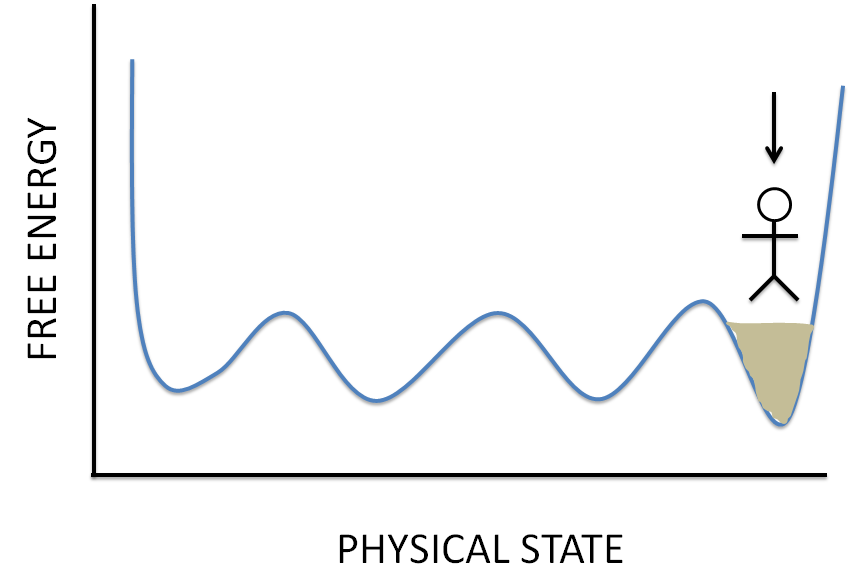
\includegraphics[width=3in]{figures/wl.png}
        \caption{The Wang-Landau and $1/t$ algorithms only add ``dirt'' to one hole at a time, when the state corresponding to that hole is visited.}
        \label{fig:wl}
    \end{center}
\end{figure}

\subsection{\label{sec:multiplestatemethods}Multiple State Reweighting Methods}

The Wang-Landau and its $1/t$ variant only update one state's free energy at one time, i.e. when it is visited during the random walk in the expanded ensemble.  However, in theory, it should be possible to update the weights of multiple states the same time.

\subsubsection{\label{sec:transition_matrix}Transition Matrix Monte Carlo Approaches}

Assume we use some Monte Carlo approach to sample between neighboring state $i$ and $j$.  The probability of ending up in state $i$ or state $j$, computed during the transition process, can also be accumulated and used to calculate free energies {\color{red}fill in more details here, see
for example~\cite{siderius_2013}}. Any transition kernel preserving detailed balance, either nearest neighbor, or all-state, can be used to calculate free energies either after a fixed weight simulation.

A collection matrix $C$ is constructed of transitions from state $i$ to $j$; we update the row $C_{i,j}$ for all $j$, if we are currently in $i$.

It can be updated with: 
\begin{enumerate}
\item Actual transitions \label{item:actual}
\item Actual proposals and the acceptance probability, independent of the algorithm used to accept the proposed move.\label{item:proposal}
\item The total transition's probability, independent of the algorithm actually used to perform the move. \label{item:transition}
\end{enumerate}

We give examples of all cases.
 
In case~\ref{item:actual}, then if one is in state $i$, and a transition to $j$ is accepted (by whatever detailed-balance preserving algorithm is used), then $C_{i,j}$ is incremented by one.

In case~\ref{item:proposal}, if one is using standard nearest-neighbor Metropolis Monte Carlo, with a move probability of 50\% up and 50\% down, then whenever a move up to state $i+1$ is proposed then
$C_{i,i+1}$ is incremented by $p(x,i \rightarrow i+1) =
\mathrm{min}(1,e^{-u_{i+1}(x)+u_i(x)})$, and $C_{i,i}$ is incremented by $1-p(x,i \rightarrow i+1)$, regardless of whether or not the
estimate is accepted or rejected.  If the Barker transition
probability is used for incrementing (even if the Metropolis transition probability was used to test the actual transition), then
$C_{i,i+1}$ is incremented by $p(x,i\rightarrow i+1) =
\frac{e^{-u_{i+1}}}{e^{-u_{i+1}(x) + e^{-u_i(x)}}}$ and $C_{i,i}$ is
incremented by $1-p(x,i\rightarrow i+1) =
\frac{e^{-u_{i}}}{e^{-u_{i+1}(x) + e^{-u_i(x)}}}$.  If one uses
independence sampling, then each of $C_{i,j}$ is incremented by
$p(x,i \rightarrow j) = \frac{e^{f_i-u_i}}{\sum_k N_k e^{f_k-u_k}}$.

[There is a general statement somewhere showing that Metropolis
  criteria is better for transitions, and Barker criteria is better
  for calculating free energies.  Related to some of Peskin's seminal
  paper proving metropolis is better than Barker. Will need to dig it out.]

We finally consider the case of ~\ref{item:transition}. If using nearest neighbor MC, then if we were at state $i$, at each iteration we update:
Using a Gibbs sampling move, then the transition kernel would be:
\begin{eqnarray}
C_{i,i-1} &+=& \frac{1}{2}\mathrm{min}(1,e^{-u_{i-1}(x)+u_i(x)})\\ 
C_{i,i} &+=& 1 - \frac{1}{2}\left[\mathrm{min}(1,e^{-u_{i-1}(x)+u_i(x)}) + \mathrm{min}(1,e^{-u_{i+1}(x)+u_i(x)})\right]\\ 
C_{i,i+1} &+=& \frac{1}{2}\mathrm{min}(1,e^{-u_{i+1}(x)+u_i(x)})
\end{eqnarray}

Once the matrix is accumulated, we can then calculate the free energies.  The probability matrix $P_{i,j}$ is simply the collection matrix with each row normalized by the amount of time (measured in interval between samples) spent in each state $j$. Detailed balance states that the ratio of probabilities from $i\rightarrow j$ and from
$j \rightarrow i$ is equal to the ration of the equilibrium
properties, which can be expressed as:
\begin{eqnarray}
e^{-f_i+f_j} = \frac{P_{j,i}}{P_{i,j}} 
\end{eqnarray}

From Bennett's original paper and further analysis by Shirts and Chodera, we know that we can calculate the free energy from
\begin{eqnarray}
e^{-(f_i-f_j)} = \frac{\expect{\alpha_{ij}(x) e^{-u_i(x)}}_j}{\expect{\alpha_{ij}(x) e^{-u_j(x)}}_i}
\end{eqnarray}
With $\alpha_{ij}(x)$ an arbitrary function that is nonzero everywhere
on $x$. If we are using Barker the estimator to benchmark transitions, we have:
\begin{eqnarray}
e^{-(f_i-f_{i+1})} &=& \frac{P_{j,i}}{P_{i,j}} \\
                   &=& \frac{\expect{\frac{e^{-u_{i}}}{e^{-u_{i+1}}+e^{-u_i}}}_{i+1}}{\expect{\frac{e^{-u_{i+1}}}{e^{-u_{i+1}}+e^{-u_i}}}_i}
\end{eqnarray}

This can be seen as a solution to the generalized Bennett formulation
with $\alpha_{ij} = \frac{1}{e^{-u_{j}}+e^{-u_i}}$. The optimal
$\alpha_{ij}$ for two states is:
$\alpha_{ij} = \frac{N_j e^{f_j}}{N_i e^{f_i-u_{i}}+ N_j f_j e^{-u_j}}$
% this is from the Shirts & Chodera formulation; check to make sure
% it's equivalent to the Bennett formulation without any additional assumptions.
%\alpha_{ij} = \frac{N_j e^{f_j}}{N_i e^{f_i-u_{i}}+ N_j f_j e^{-u_j}}
%            =  \frac{1}{N_i/N_j e^{f_i/f_j-u_{i}}+ e^{-u_j}}
Thus, the Barker method with transition matrix MC will be equivalent in efficiency in the optimal limit of $N_i \approx N_j$ and $f_i \approx f_j$, but will eventually give the correct free energy difference $f_i = f_j$ regardless.  

Let's analyze further the difference between Bennett's formalism for free energies, and the transition matrix MC formalism. 

Transition matrix MC calculates free energies.
\begin{eqnarray}
e^{-f_i+f_j} = \frac{P_{j,i}}{P_{i,j}} 
\end{eqnarray}

While Bennett's formalism is that:
\begin{eqnarray}
e^{-(f_i-f_j)} = \frac{\expect{\alpha_{ij}(x) e^{-u_i(x)}}_j}{\expect{\alpha_{ij}(x) e^{-u_j(x)}}_i}
\end{eqnarray}
Clearly, $P_{j,i} = \expect{P_{ji}(x)}_j$ is an average over configurations from the $j$th
state, as it is an average of the incremented transition probabilities
leaving from the $j$th state.

So, in this case $P_{ji}(x) = \alpha_{ij}(x) e^{-u_i(x)}$ and $P_{ij}(x) = \alpha_{ij}(x) e^{-u_j(x)}$. So any set of transition functions will work as long as $\frac{P_{ji}(x)}{P_{ij}(x)} = e^{u_j(x)-u_i(x)}$, which Barker, Metropolis, and independence
sampling do.  Indeed, this just statement of detailed balance in sampling in state space when restricted to a single $x$ (maybe something else as well).

What would a transition matrix MC method look like with optimally efficient calculations? Let's assume first only two states, and assign a weight $\eta_i$ to each state $i$.  Transitions between weights
using the Barker formalism would be 
\begin{equation}
P_{ji}(x) = \frac{e^{\eta_i-u_i(x)}}{e^{\eta_i - u_i(x)} + e^{\eta_j - u_j(x)}}
\end{equation}
If $\eta_i/\eta_j = N_j/N_i e^{f_i-f_j}$, then we obtain the optimal
variance estimator, although the ratio $P_{i,j}/P_{j,i}$ will now be
equal to $e^{-(f_i-\eta_i) + (f_j - \eta_j)}$, as the weights of each
state have changed.

Of course, to do this, it requires knowing the free energies ahead of
time, and would require adjusting the weights to the current $N_i$ and
$N_j$ at each step of the simulation, which is not really supported in
the Transition Matrix Monte Carlo formalism, as time symmetry is
broken, and steps backwards would not be equal to steps forward in
state space.

Finally, we note that with the definition of transition matrix free energies, we get:
\begin{eqnarray}
e^{-f_i+f_j} = \frac{P_{j,i}}{P_{i,j}} 
\end{eqnarray}

Which is equivalent up to normalization:
\begin{eqnarray}
f_i = -\ln P_{j,i} = -\ln \sum_{n=1}^{N_i} C_{ji}(x_n) - \ln N_i\\ 
f_j = -\ln P_{i,j} = -\ln \sum_{n=1}^{N_j} C_{ij}(x_n) - \ln N_j
\end{eqnarray}

In the limit of large $N_i$, since $\ln(x+\delta x) = \ln(x) + \ln\left[1 +
  \frac{\delta x}{x}\right] \approx \ln(x) + \frac{\delta x}{x}$, and $\frac{N_i}{N_{i-1}} \approx 1$, we
have:

\begin{eqnarray*}
\Delta f_i &=& f_{i,n} - f_{i,n-1} \\
           &=& -\ln \left[ \frac{\sum_{n=1}^{N_j} C_{ji}(x_{n})}{N_i}\right] - f_{i,n-1} \\
           &=& -\ln \left[ \frac{\sum_{n=1}^{N_i-1} C_{ji}(x_{n})}{N_i-1}\frac{N_i-1}{N_i} + \frac{C_{ji}(x_{N_i})}{N_i} \right] - f_{i,n-1} \\
           &=& -\ln \left[e^{-f_{i,n-1}}\frac{N_i-1}{N_i} + \frac{C_{ji}(x_{N_i})}{N_i-1}\frac{N_i-1}{N_i}\right] - f_{i,n-1} \\
           &=& f_{i,n-1} + \ln \left[1 + \frac{C_{ji}(x_{N_i})e^{f_{i,n-1}}}{N_i}\right] - f_{i,n-1}\\
           &=& \frac{1}{N_i} C_{ji}(x_{n})e^{f_{i,n-1}}
\end{eqnarray*}
If $C_{ji}$ is incremented with the Barker ratio, then Transition
Matrix Monte Carlo would be equivalent to incrementing the free energy
by:
\begin{eqnarray}
\Delta f = \frac{1}{N_i} \frac{e^{f_{i,n-1}-u_i(x)}}{e^{-u_i(x)} +
  e^{-u_j(x)}}
\end{eqnarray}
Which can be compared to other incrementing methods discussed later.
 
\subsubsection{\label{sec:awh}Accelerated Weight Histogram}

We can also update all weights simultaneously by reweighting the information gathered at the current state.  One such method is the 'Accelerated Weight Histogram' (AWH) method of Lidmar
\cite{Lidmar2012}.  In the AWH algorithm, a certain amount of configurational sampling ($N_x$ times) is performed, the Gibbs sampler is used to move between states, and a histogram of weights for each state is accumulated.  These three steps are repeated a certain number
$N_I$ times.  Afterwards, the weight histogram is used to update the free energy weights and the histogram is updated once more.  This sequence constitutes one 'iteration' and the entire process is repeated a certain number of times, or until a certain accuracy is reached if the analytical weights are known.  The entire algorithm is described as follows:

After $N_x$ configurational updates following $\pi(x,k)$: a new state $j$ is proposed by the Gibbs sampler probabilities $\alpha(j|x, i)$:

\begin{equation}\label{eq:gibbsproposal}
  \alpha(j|x, i) = \pi(i|x)
\end{equation}
where $\pi(i|x)$ is given in Equation~\ref{equation:expanded-ensemble-gibbs-update}.  This new state $j$ is always accepted.  The previous state $i$ is allowed as a proposal for $j$ under this scheme.  The weight histogram is then updated by the computed $\pi(i|x)$ weights:

\begin{equation}
h_{\mathrm{new}}(i) = h_{\mathrm{old}}(i) + \pi(i|x)
\label{eq:awh-weight-histogram}
\end{equation}

Once those steps have been repeated $N_I$ times, the free energy parameters are updated according to:

\begin{equation}
g_{i,\mathrm{new}} = g_{i,\mathrm{old}} - \ln{\frac{h_{\mathrm{new}}(i)K}{N}}
\label{eq:awh_free_energy_up}
\end{equation}

where $N$ is the total number of samples collected up to that point.  The entire procedure is then repeated.
\subsubsection{Self-adjusted mixture sampling}
Ziqiang Tan independently developed what was called Self-adjusted mixture sampling~\cite{SAMS:2014}.  Although the notation is quite different, one can define take eq. 12, which states:
\begin{equation}
\xi^{(t-\frac{1}{2})} = \xi^{(t-1)} + t^{-1}\left\{w_i(X_t);\xi^{(t-1)})/\pi_i,...,w_m(X_t;\xi^{(t-1)})/\pi_m\right\}^T
\end{equation}
Translating from Tan's
terminology, $t$ is the current step of MC/MD sampling, the $\xi^(t-\frac{1}{2}$ is the vector of $g_{i,new}$ and $\xi^{t-1}$ is the vector of $g_{i,old}$. $X_t$ is the same as $x$ in the current terminology, and and $\pi_i$ are the target probability distributions of each state; if we assume we are looking for equal sampling of the states, they are all simply equal to 1; we will look at other variations later. $w_j(X;\xi)$ is the expectation of the Monte Carlo transition probability to state $j$ states when the current configuration is $X$, and the current weights are $\xi$. If we use the Gibbs transition rule, this is $\pi(i,x)$. We then have the rule:
\begin{eqnarray}
g_{i,new} = g_{i,old} - t^{-1}\pi(i,x)
\end{eqnarray}

\if 0
\subsection{\label{sec:general}A general formalism}

General formalism of all the methods 

\begin{itemize}
\item Run $N_r$ steps with a given weight

\item Update using the data; either all data so far, or only the last $N_r$ points.

\item If using all the data, can either:
\begin{itemize}
  \item Compute free energies by ratios
  \item Compute free energies by BAR
  \item Compute by all state reweighting (MBAR -- theoretically optimal).
\end{itemize}

\item if using only the most recent data, compute with some sort of differential update.  And weight this updated according to the data sampled.
\begin{itemize}
  \item using only the last data point
  \begin{itemize} 
  \item Either WL, or transition matrix, or weighted WL
  \item if weighted WL \begin{itemize}
  \item update with $\delta \pi(i,k)$
   \item do we linearize or not?
       %Nexp(-g_k) + \delta \pi(i,k)
       %new is g_k = log[Nexp(g_k)+\delta \pi(i,k)]
       %            log[Nexp(g_k)(1+[\delta \pi(i,k)/exp(g_k)])]
        %          = g_k+lnN + log (1 + \delta(\pi(i,k)/exp(g_k))
         %         = g_k+lnN + \delta(\pi(i,j)/Nexp(g_k))
          %        = g_k + 1/N \delta(\pi(i,j)

  \item need to figure out what $\delta$ is. Is some function of the current weights. Generally should weight the data according to the amount of data sampled -- hence should scale with $1/t$.
  \end{itemize}
  \end{itemize}
  \item using last $N$ data points
   \item \begin{itemize}
    \item $p(i,i)$ use ratios
    \item $p(i,i+1)$ use BAR
    item all $p(i,j)$ use MBAR
   \end{itemize}

    \item How to weight these last $N$ points?
     \begin{itemize} 
       \item do we assume that the $N_k's$ in THIS set are equal, or not?
       \item do we assume that the $N_k's$ in the PREVIOUS set are equal, or not?  Does it even matter?
     \end{itemize}
  \item Switching.  When do we shift between the various regimes?
\end{itemize}
\item If only using the most recent data, the optimal strategy will change
depending on whether it's new data or old data.

\item (How are histograms used in bookkeeping?)
\end{itemize}
\fi

\subsection{\label{sec:design}Designing a Free Energy based Expanded Ensemble Algorithm}
In this section, we review the basic components of any expanded ensemble weight determination method for dynamic estimation for a set of $K$ thermodynamic states in Monte Carlo simulations.  We use the original algorithm proposed by Wang and Landau \cite{wang-landau:prl:2001:wang-landau}, the $1/t$ update to the Wang-Landau algorithm proposed by Belardinelli and Pereyra \cite{Belardinelli2008}, and the recently developed 'Accelerated Weight Histogram' (AWH) method of Lidmar \cite{Lidmar2012} as examples.

\subsubsection{Initial Guess for Weights}
In any of these class of methods the weights are \emph{a priori} unknown.  Therefore, an initial guess is needed.  An initial estimation scheme could be used, estimates from a different simulation could be used, or the free energies can all be set to zero $g_k = 0$.  In the original Wang-Landau algorithm and the $1/t$ method, the initial guesses are all zero $g_k = 0$.  In the Accelerated Weight Histogram method, Lidmar presents a bootstrapping scheme that works essentially as a version of the full AWH method with small numbers of sampling (10-100) and iterations(100-1000).  Finally as Lidmar advises, free energy estimates from another method, like the Wang-Landau method can be used as an initial guess to improve upon in the current simulation.

%MRS:
Our general approach is that we would like any method to be self-starting, i.e. we don't need to do any manual editing of parameters in an initial phase.  Our method should lead to convergence in all but particularly pathological cases  Any initial phases should be ended automatically, rather than by human intervention.  The method should be independent of initial estimate of $g_k$, i.e. it will converge to the correct $g_k$ with any physically rational choice of weights (i.e. setting one to $-10^6$ and the rest to zero is probably unreasonable).

\subsubsection{Updating the Free Energies: Frequency of Configuration/State Sampling}
Another question in the design of these algorithms concerns the frequency at which moves on configuration and state spaces are performed.  A higher frequency of moves in configuration space could help prevent free energies from becoming trapped in local minima and saturation of error.  Furthermore, one must decide whether to alternate between configuration and state moves, or whether to make steps in configuration and state spaces randomly.  An alternating scheme satisfies balance, whereas a random scheme satisfies detailed balance.  An advantage of the alternating scheme could be used for on-the-fly estimation of expectation values.

%MRS: perhaps we don't need to decide this. This will depend on the nature of the system. A general principle is that things should converge as long as configuration and state space sampling is uncorrelated.  So perhaps we just need to assume we know the correlation times of the system, and alternate (or randomly choose) with that frequency.

\subsubsection{Updating the Free Energies: How Often?}
As described earlier, a joint random walk in configuration and parameter spaces is performed, subtracting some $\Delta g_k$ from the sampled state's or all states' free energies as the simulation proceeds.  The difference between most expanded ensemble algorithms is how to perform this subtraction. First to decide, is how often to perform these subtractions, i.e. is it done after every move in state space, or after a certain number of them?  In the original Wang-Landau method and $1/t$ methods, the free energies are updated after each move in state/parameter space.  However, in the AWH method, $N_I$ samples are collected to accumulate weights for each state in a histogram before updating the free energy parameters.

%MRS: I don't have a good sense for this.  If the weights change faster than the correlation times to go between configuration states, then the simulation could get stuck.  But I don't know a mathematical way to express this right off.  We may have to experiment.

\subsubsection{Updating the Free Energies: What is $\Delta g_k$ as a function of $k$?}

The value of $\Delta g_k$ by must be determined at each step, For example some methods use reweighting to update all states' free energies and others just update that of the sampled state when a step in state space is performed.  In the Wang-Landau, only the current state is updated, and by a fixed increment \cite{wang-landau:prl:2001:wang-landau} that is reduced during the simulation.  However, reweighting can be used to update all states by a state dependent factor $\Delta g_k$, simultaneously \cite{Lidmar2012}.  Whatever the update scheme, the long time behavior should exactly satisfy the $1/t$ behavior observed by Belardinelli and Pereyra \cite{Belardinelli2008,Lidmar2012}.

%MRS: I need to think about this a little.  The question is, is this another way of phraseing the next item?  I'm not sure.

\subsubsection{Updating the Free Energies: When to reduce $\Delta g_k$}
The value of $\Delta g_k$ must be decreased throughout the simulation in order to make the free energy estimates $g_k$ converge as the simulation proceeds.  The frequency with which this is done and to what decrease $\Delta g_k$ by must be determined.  In the original Wang-Landau algorithm, a histogram keeps track of the times a state was visited since the last time the free energy increment was scaled.  The $\delta $ increment, the same for all states, was halved every time this histogram was flat, i.e. $tolerance \geq (max(h)-avg(h))/avg(h)$.  The histogram was then reset to zero and rebuilt over time until the next flattening event. However, scaling by one-half leads to a saturation of error, and the long time scale behavior of the scaling factor was shown to be proportional to $1/t$, where $t$ is the Monte Carlo time. \cite{Belardinelli2008}.  In the AWH method, a histogram of Gibbs sampling weights is accumulated and never reset to zero.  Since the free energy update in the AWH method goes as the $-\ln{h_i(K/N)}$, the growing histogram makes the free energy updates smaller and allows for convergence.

With these criteria in mind, we continue with the derivation of our proposed algorithmic modifications.
\begin{comment}
Free Energy EXE Methods overview

What are the variables:

1. f_k is zero everywhere to start.
2. At each step, add delta f_k to all k   - difference between all methods how do you do that?

  a. Do you add delta f_k everytime you make a step in k?
       i. OWL -- every time you make a step in state.   WE STAY WITH THIS.
       ii Lidmar every N_I (100-1000 parameter moves during initial stage)  ( I need to look paper point)
       %MRS: we may want to try this out

  b. Do you make steps in k very frequently compared to steps in configuration?
      i. we do, maybe we are doing it wrong?  Probably more steps in configuration.
      ii. Do we alternate, or make random steps?  Alternating obeys balance, random obeys detailed balance?  Are there advantages and disadvantages STICK WITH RANDOM, try 90% config / 10% state.
      %MRS: should be determined by the correlation time.  Of course, the question is WHICH correlation time? The configuration correlation time at the current state?  If we are below the freezing transition, that could take forever.  Perhaps it is then the minimum of the correlation time of the state and the configuration time?  Let's think longer.
   c. When do you reduce delta f_k ?
             OWL -- lower delta f_k every time a histogram is flat
                 a histogram keeps track of times visited since the last time scaling is done.
             1/t always --  every step.
              Lidmar --
         We are pretty sure that 1/t is correct long time scale
         %MRSL agreed! THough there might be other ways to do it.

    d. How much do you reduce delta f_k by?
             OWL -  lower delta f_k by constant scaling factor
            1/t - lower delta f_k  a t/ t+1 scaling factor
      Pretty sure that long term, 1/t is right way.
      %MRS: yes.

    e. What is delta f_k it as a function of states?
     OWL  delta f_k is  WLDELTA if current state, 0 if other states
     WWL  delta f_k is propto exp(f_k-u_k) / [sum k’ N_k’ *exp(f_k’-u_k’)]

    We’re pretty sure that ours is correct (exactly equal) for long term.
    %MRS: yes.

3. When do you stop?  (probably doesn’t matter as much)
    %MRS: right, depends on what you want.

\end{comment}
%\subsubsection{Gibbs Sampling}

\subsection{\label{sec:wwl}A weighted Wang-Landau method}

The Wang-Landau algorithm is useful, but information can only be collected from one state at a time.  If we are visiting all the states, nearby states sample similar phase space.  There must be some way to use information sampled at each state to gain information about the other states nearby.  We seek a Wang-Landau like algorithm with a basis in multistate reweighting techniques.  This way, when a state is visited, information on all of the possible states can be updated by a weighted amount.  We start with MBAR, the provably minimum variance free energy estimator given $N_{i}$ samples from each of $i=1 \ldots K$ states. \cite{shirts-chodera:jcp:2008:mbar}.  The estimator for the reduced free energy for each state $f_{i}$ up to an additive constant is given by the following self-consistent equation \cite{shirts-chodera:jcp:2008:mbar}:

\begin{eqnarray}
\exp(-f_i) = \sum_{n=1}^N \frac{\exp(-u_i(x_n))}{\sum_k N_k \exp(f_k-u_k(x_n))}
\label{eq:MBAR}
\end{eqnarray}

Assuming that after $n$ steps of simulation that we have a decent estimate of the free energies $\hat{f}_{i}$ and that we wish to add one more sample without recalculating the free energies explicitly:
\begin{eqnarray}
e^{-\hat{f}_{i}^{(N)}} &=& \sum_{n=1}^N \frac{\exp(-u_i(x_n))}{\sum\limits_k N_k \exp(\hat{f}_{k}^{(n)}-u_k(x_n))} \nonumber \\
e^{-\hat{f}_{i}^{(N+1)}} &=& \sum_{n=1}^N \frac{\exp(-u_i(x_n))}{\sum\limits_k N_k \exp(\hat{f}_{k}^{(n)}-u_k(x_n))} +  \nonumber \\
                          & & \frac{\exp(-u_i(x_{N+1}))}{\sum\limits_k N_k \exp(\hat{f}_{k}^{(N+1)}-u_k(x_{N+1}))}  \nonumber \\
e^{-\hat{f}_{i}^{(N+1)}} &=& e^{-\hat{f}_{i}^{(N)}} + \frac{\exp(-u_i(x_{N+1}))}{\sum_k N_k \exp(\hat{f}_{k}^{(N+1)}-u_k(x_{N+1}))} \nonumber \\
   &=& e^{-\hat{f}_{i}^{(N)}} \left[1 + \frac{\exp(\hat{f}_{i}^{(N)}-u_i(x_{N+1}))}{\sum_k N_k \exp(\hat{f}_{k}^{(N+1)}-u_k(x_{N+1}))}\right] \nonumber \\
\hat{f}_{i}^{(N+1)} &=& \hat{f}_{i}^{(N)} - \ln\left[1 + \frac{\exp(\hat{f}_{i}^{(N)}-u_i(x_{N+1}))}{\sum_k N_k \exp(\hat{f}_{k}^{(N+1)}-u_k(x_{N+1}))}\right] \nonumber \\
                   &\approx& \hat{f}_{i}^{(N)}- \frac{\exp(\hat{f}_{i}^{(N)}-u_i(x_{N+1}))}{\sum_k N_k \exp(\hat{f}_{k}^{(N)}-u_k(x_{N+1}))}
\end{eqnarray}
In the last step, we make two approximations.  First, the logarithm is expanded in the first order Taylor series in the limit of large numbers of samples, so that $\ln (1-x) \approx -x$.   Second, in the denominator, we approximate the unknown $\hat{f}_{i}^{(N+1)}$ by $\hat{f}_{i}^{(N)}$.  The sum over $N_k$, however, does include the new data point, so that $\sum_k N_k = N+1$.
This formula based on MBAR gives us a way to update the free energies at each state during am expanded ensemble simulation.

We note that this is exactly Zhiqiang Tan's optimal (Eq. 12 in the version of the draft I've been reading), obtained in a different manner (fill in the blanks).

% ------Is it possible to linearize? So far, haven't been able to ----------------------
%{\color{red}[JDC: You're also omitting the contribution from reoptimizing $f_k$ on the old data, the left-hand term involving the sum from $n=1$ to $N$ on the left-hand side of the first equation.  It's not clear to me that this contribution is not as large as the contribution from the new data point $N+1$.  I would be much happier if you could linearize \emph{both} the old sum from $n=1$ to $N$ \emph{and} the contribution from $N+1$ and solve for the updated $f_{i,new}$ using this linearized form.]}
% MRS: this looks like it reduces to a system of quadratic equations, so I don't know that it can be solved easily.  However
% it is probably a good idea to find the leading term in the approximation to see how big an effect each of the approximations has.
%---------------------------------------------------------------------------------------

At large numbers of total samples $N$, all states in the expanded ensemble will be visited approximately equally, with $N_{k} \approx N/K$ for all K. In the large-$N$ limit we therefore can write this approximately as:
\begin{eqnarray}
\hat{f}_{i}^{(N+1)} \approx \hat{f}_{i}^{(N)}- \frac{1}{N}\frac{\exp(\hat{f}_{i}^{(N)}-u_i(x_{N+1}))}{\frac{1}{K}\sum_k \exp(\hat{f}_{k}^{(N)}-u_k(x_{N+1}))}
\end{eqnarray}
Clearly the exponential terms in the numerator and the denominator are of the same magnitude, so the accumulation term is proportional to the number of samples collected so far, rather than a fixed number, as suggested in the original Wang-Landau
algorithm.  Interestingly, this is exactly the proposed accumulation
factor for the $1/t$ algorithm proposed by~\citet{Belardinelli2007},
which states that the incrementor factor $\delta$ should
asymptotically approach $K/N$. In that method, they start with the $\delta$
incrementor being scaled by $1/2$ each time, and when $1/t$ is
larger, they switch over to $1/t$.

So at each step, we have a formula based on MBAR for how to update the free energy in an adaptive manner given the information collected so far.  To turn this into an all-state Wang-Landau-like algorithm, however, we need to have some way to compute a histogram to determine
when the weights lead to sufficient flatness.  We could use a simple discrete histogram update, as in the original Wang-Landau algorithm. However, if we are computing the energies at all other states, we could update all states by a weighted amount.  For example, we could look at the conditional probability for $k$ give the sample $x$ given
by:
\begin{eqnarray}\label{eq:pi(k|x)-2}
\pi(i | x) &=& \frac{e^{g_k}q_i(x)}{\sum\limits_{k=1}^K e^{g_{k}}q_{k}(x)} = \frac{e^{g_i - u_i(x)}}{\sum\limits_{k=1}^K e^{g_{k} - u_{k}(x)}} .
\end{eqnarray}
This is the probability of a state $i$ given sampling from $x$.
Therefore, we can interpret it as amount we should increment each
state $i$ when we perform a sample from any state, so we now have a
way to interpret the histograms.

To make the entire process more compact, we define the quantity
\begin{eqnarray}
\pi(i|N,x) = \frac{N_k\exp(f_i-u_i(x))}{\sum_k N_k \exp(f_k-u_k(x))}
\end{eqnarray}
Which closely resembles $\pi(i|x)$, and equals it in the limit where
all $N_k$ are equal, but takes into account the inequal weighting so
far.

This can be generalized to arbitrary weights $g_k$ that differ from
$f_k$ by $\Delta_k$.  This would be the case if we wish to sample
state $i$ by more than equal sampling proportional to
$\exp(\Delta_i)$.
\begin{eqnarray}
\pi(i|x,\vec{N},\vec{\Delta}) = \frac{N_k\exp((g_i-\Delta_i)-u_i(x))}{\sum_k N_k \exp((g_k-\Delta_k)-u_k(x))}
\end{eqnarray}
Where $\vec{N}$ is the list of all numbers of samples from each state
$N_k=1,\ldots,k$, and $\vec{\Delta}$ is the vector of all deviations
of the weights from equal sampling.

Given these definitions, we can define a new algorithm for iterative
updating of the weights and free energies by:
\begin{eqnarray}
h_{i,\mathrm{new}} = h_{i,\mathrm{old}}+\pi(i|x) \\
g_{i,\mathrm{new}} = g_{i,\mathrm{old}} - \delta \pi(i|x,\vec{N},\vec{\delta})
\end{eqnarray}
Where $\delta$ is a scaling factor that is decreased throughout the simulation.  At the point where $h_i $ reaches a certain flatness level, we ignore the histogram and scale $\delta$ as $K/N$ as in the $1/t$ algorithm of~\citet{Belardinelli2007}.  At the point when
$\delta < K/N$, we ignore the histogram, set $\delta = K/N$ at each
step, and simply update the free energies, as in the $1/t$ algorithm.
%\textcolor{red}{ACK: Since we are switching to $1/t$ after the first flat histogram, I think it would be a good idea to cite a math study saying $1/t$ is the way to go.}
\begin{eqnarray}
\exp(-f_i) = \sum_{n=1}^N \frac{\exp(-u_i(x_n))}{\sum_k N_k \exp(f_k-u_k(x_n))}
\label{eq:MBAR}
\end{eqnarray}
\begin{comment}
[MRS: note: can we do something with linear response theory and come
  up with results that hold near equilibrium? It seems that for most
  adaptive methods, once we are a decent way into the algorithm, then
  we are going to be in the linear regime as we adjust weights; we
  will be almost at equilibrium].
\end{comment}
\if 0
\subsection{\label{sec:ambar}Approximate MBAR}
In this section, we derive an update to estimates of weights for a set of macrostates using an approximate MBAR formalism.

Assuming that after $N$ new steps of simulation, a step being a state transition, that we have a decent estimate of the free energies $\hat{f}_{i}$ and that we wish to add $N_I$ more samples without recalculating the free energies explicitly using MBAR. This approximate formalism reweights data from only the last $N_I$ state trials, not over the entire time history, $N+N_I$:

We start with the definition of the previous weights, $f_{i}^{(N)}$
\begin{equation}
e^{-\hat{f}_{i}^{(N)}} = \sum_{n=1}^N \frac{\exp(-u_i(x_n))}{\sum\limits_k N_k \exp(\hat{f}_{k}^{(n)}-u_k(x_n))}
\end{equation}

Then we update the old weights by the term on the far right below:
\begin{equation}
e^{-\hat{f}_{i}^{(N+N_I)}} = \sum_{n=1}^N \frac{\exp(-u_i(x_n))}{\sum\limits_k N_k^{old} \exp(\hat{f}_{k}^{(n)}-u_k(x_n))} +
                           \sum_{n=N}^{N+N_I} \frac{\exp(-u_i(x_{n}))}{\sum\limits_k N_k^{new} \exp(\hat{f}_{k}^{(n)}-u_k(x_{n}))}
\end{equation}
Substituting for the first term on the righthand side with the old free energy terms:
\begin{equation}
e^{-\hat{f}_{i}^{(N+N_I)}} = e^{-\hat{f}_{i}^{(N)}} + \sum_{n=N}^{N+N_I}\frac{\exp(-u_i(x_{n}))}{\sum_k N_k \exp(\hat{f}_{k}^{(N+N_I)}-u_k(x_{n}))}
\end{equation}
Then we factor out $e^{-\hat{f}_{i}^{(N)}}$:
\begin{equation}
e^{-\hat{f}_{i}^{(N+N_I)}} = e^{-\hat{f}_{i}^{(N)}} \left[1 + \sum_{n=N}^{N+N_I} \frac{\exp(\hat{f}_{i}^{(N)}-u_i(x_{n}))}{\sum_k N_k \exp(\hat{f}_{k}^{(N+N_I)}-u_k(x_{n}))}\right]
\end{equation}
Lastly, we take the natural log of both sides and divide both sides by -1.
\begin{equation}
\hat{f}_{i}^{(N+1)} = \hat{f}_{i}^{(N)} - \ln\left[1 + \sum_{n=N}^{N+N_I} \frac{\exp(\hat{f}_{i}^{(N)}-u_i(x_{n}))}{\sum_k N_k \exp(\hat{f}_{k}^{(N+1)}-u_k(x_{n}))}\right] \nonumber \\
\end{equation}
\fi

\subsection{\label{sec:wwl}Comparison to Accelerated Weight Histogram}

Assuming that after $n$ steps of simulation that we have a decent estimate of the free energies $\hat{f}_{i}$ and that we wish to add $N_I$ samples without recalculating the free energies explicitly.  We also assume that all states have been visited with approximately equal probability, so that $N_k \approx N/K$, and we call $\Delta \hat{f}_i = \hat{f}_{i}^{(N+N_I)} - \hat{f}_{i}^{N}$.

Then:
\begin{eqnarray}
e^{-\hat{f}_{i}^{N}} &=& \sum_{n=1}^N \frac{\exp(-u_i(x_n))}{\sum\limits_k N_k \exp(\hat{f}_{k}^{N}-u_k(x_n))} \nonumber \\
e^{-\hat{f}_{i}^{N+N_I}} &=& \sum_{n=1}^{N} \frac{\exp(-u_i(x_n))}{\sum\limits_k N_k \exp(\hat{f}_{k}^{N}-u_k(x_n))} +  \nonumber \\
                          & & \sum_{n=1}^{N_I} \frac{\exp(-u_i(x_{n}))}{\sum\limits_k N_k \exp(\hat{f}_{k}^{N}-u_k(x_{n}))}  \nonumber \\
                          &=& \sum_{n=1}^{N} \frac{\exp(-u_i(x_n))}{\sum\limits_k \frac{N+N_I}{K}\exp(\hat{f}_{k}^{N}-u_k(x_n))} +  \nonumber \\
                          & & \sum_{n=1}^{N_I} \frac{\exp(-u_i(x_{n}))}{\sum\limits_k \frac{N+N_I}{K} \exp(\hat{f}_{k}^{N}-u_k(x_{n}))}  \nonumber \\
                          &=& \frac{N}{N+N_I}\sum_{n=1}^{N} \frac{\exp(-u_i(x_n))}{\sum\limits_k \frac{N}{K}\exp(\hat{f}_{k}^{N}-u_k(x_n))} +  \nonumber \\
                          & & \frac{K}{N+N_I}\sum_{n=1}^{N_I} \frac{\exp(-u_i(x_{n}))}{\sum\limits_k \exp(\hat{f}_{k}^{N}-u_k(x_{n}))}  \nonumber \\
                          &=& \frac{N}{N+N_I}\exp(-\hat{f}_{k}^{N}) + \frac{K}{N+N_I}\sum_{n=1}^{N_I} \frac{\exp(-u_i(x_{n}))}{\sum\limits_k \exp(\hat{f}_{k}^{N}-u_k(x_{n}))}  \nonumber \\
\exp(-\Delta f)           &=& \frac{N}{N+N_I} + \frac{K}{N+N_I}\sum_{n=1}^{N_I} \frac{\exp(f_{k}^{N}-u_i(x_{n}))}{\sum\limits_k \exp(\hat{f}_{k}^{N}-u_k(x_{n}))} \nonumber \\
                          &=& \frac{K}{N+N_I}\left[\frac{N}{K} + \sum_{n=1}^{N_I} \frac{\exp(f_{k}^{N}-u_i(x_{n}))}{\sum\limits_k \exp(\hat{f}_{k}^{N}-u_k(x_{n}))}\right]  \label{eq:NIsum}
\end{eqnarray}
We note that this is equivalent to Lidmar's formula for updating, because at step $N$, the weight sum is reset to $N/K$, and the rightmost term in Eq.~\ref{eq:NIsum} is exactly the weight update term of Lidmar.

Therefore, Lidmar's adaptive histogram reweighting is similar to the
optimal approach except that the free energies are only updated every
$N_I$ steps, and $N_k = N/K$ for all states is assumed.  The optimal
``weighted'' WL estimator should therefore generally be superior.

\begin{comment}
We still must determine a reasonable point to switch to the $1/N$
formula.  This will depend on the histogram flatness.  We seek a histogram flatness criteria.

In the limit of large numbers, the distribution of histogram
probabilities will be $p_k = 1/K \pm \sqrt{K-1/NK^2}$. Assume that all
the bins are independent (they are not, since $\sum_k P_k = 1$.  The
distribution of the {\rm relative} values will have mean $r_k =
p_k/(K^{-1} = 1$ and variance $K^2(K-1/NK^2)$ = $K-1/N$.  In the limit
of large numbers of bins, we assume $K-1 \approx K$. The probability
that a given bin will have relative error $r_k$ inside some cutoff $c$
will be
\begin{eqnarray}
P_c = P(1-c < r_k < 1+c) &=& 2\int_{1}^{1+c} \sqrt{\frac{1}{2\pi \sigma^2}} e^{-\frac{(r_k-c)^2}{2\sigma^2}} dr_k\\
                   &=& 2\int_{0}^{c} \sqrt{\frac{N}{2\pi K}} e^{-\frac{Nr_k^2}{2K}} dr_k\\
                   &=& \frac{2}{\pi}\int_{0}^{\sqrt{Nc^2/2K}} e^{-t^2} dt\\
                   &=& \mathrm{erf}(Nc^2/2K)
\end{eqnarray}

The probability that {\em none} of the bins (assuming independence)
will have a value inside this range will be $1-P_c^N$.  If we set this
to some constant $C$, then we have $\mathrm{erf}(Nc^2/2K)^N = 1-C$, or
$\mathrm{erf}(Nc^2/2K) = (1-C)^{1/N}$.  For fixed $C$ and $N$, how does $c$
vary with $K$?  This seems to imply that c will scale as $sqrt(K)$

$c^2/K$ is invariant.  So if K increases by a factor of 10, then $c$
will increase by a factor of $sqrt(10)$. So if it was 0.2 before, then
it will be 0.6?
\end{comment}
In the context of the earlier ``hole'' analogy, these algorithms are illustrated in Figure~\ref{fig:wwl}
\begin{figure}
    \begin{center}
        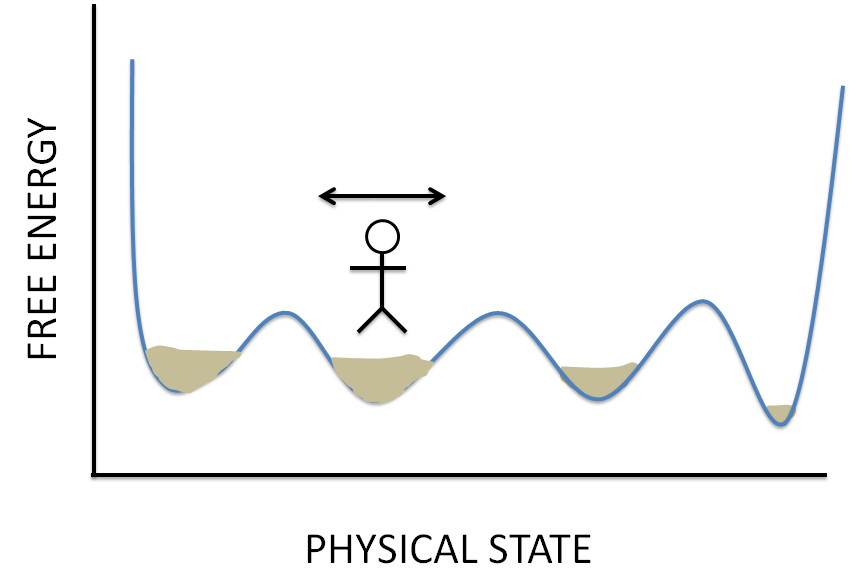
\includegraphics[width=3in]{figures/wwl.png}
        \caption{The Weighted Wang-Landau algorithms add a state-specific amount of ``dirt'' all states.  Less dirt is added to states further away from the sampled state.}
        \label{fig:wwl}
    \end{center}
\end{figure}

\subsection{Conclusions}
So, what is the recommended process at the present time?  

\begin{enumerate}
\item Run with MBAR every $N_I$ steps until it becomes computationally
unfeasible,
\item Change to the optimal self-adjusted sampling / weighted Wang-Landau method.
\end{enumerate}

\if 0
\section{State Transition Methods}
We now describe different state sampling schemes that have been used to sample the
different states in expanded ensemble simulations.  In each
algorithm, a new state $j$ is proposed given the current state $i$ and
configuration $x$.  In this study we choose at each step to sample in
either states or system configurations at a fixed probability $p$ in
order to to satisfy detailed balance, although we note that sequential
sampling schemes are
sufficient~\cite{manousiouthakis:2753:detailedbalance}.  In this study, we use independence sampling, or the Gibbs sampler, to determine transitions between states to give a fair comparison of our method against AWH, which also utilizes the Gibbs sampler.

\subsection{Metropolis }

Under the Metropolis scheme, only transitions among nearest neighbor states are allowed.  The proposed state index $j$ given the current state index $i$ is chosen to be $j = i \pm 1$ with equal likelihood.  This proposal scheme is given as:
\begin{equation}\label{eq:metproposal}
  \alpha(j| x, i) = \left\{
  \begin{array}{l l l}
    1/2 & \quad \text{if j = i -1}\\
    1/2 & \quad \text{if j = i + 1}\\
    0 & \quad \text{else}
  \end{array} \right.
\end{equation}

The proposed state $j$ is accepted with probability:
\begin{equation}\label{eq: metaccept}
  P_{\text{accept}} = \left\{
  \begin{array}{l l}
    0 & \quad \text{if $j \not\in {1,\ldots,K}$ }\\
    \min\left\{1, \frac{e^{g_j-u_j(x)}}{e^{g_i-u_i(x)}}\right\} &  \quad \text{else}\\
  \end{array} \right.
\end{equation}

A variation on this scheme is used in this paper, where the set of $K$ states lie on a torus such that states 1 and K are nearest neighbors.
\subsection{Independence Sampling}\label{sec:gibbs}
\begin{equation}\label{eq:gibbsproposal}
  \alpha(j|x, i) = \pi(i|x)
\end{equation}
where $\pi(i|x)$ is given in Equation~\ref{equation:expanded-ensemble-gibbs-update}.  This new state $j$ is always accepted.  The previous state $i$ is allowed as a proposal for $j$ under this scheme.

\subsection{Metropolized Independence Sampling}
In what we term \emph{Metropolized independence sampling} move, \cite{liu:biometrika:1996:metropolized-gibbs} a new state index $j$ is proposed from the distribution:
\begin{equation}\label{eq:metgibbsproposal}
  \alpha(j| x, i) = \left\{
  \begin{array}{l l}
    \frac{\pi(j|x, i)}{1-\pi(j|x, i)} & \quad j \neq i\\
    0 & \quad j = i
  \end{array} \right.
\end{equation}
and accepted with probability:
\begin{equation}\label{eq:metgibbsaccept}
  P_{\text{accept}}(J|x, i)= \min\left\{1, \frac{1-\pi(i|x, i)}{1-\pi(j|x, i)}\right\}
\end{equation}

This scheme has the surprising property that despite including a rejection step (unlike the independence sampling scheme of Sec.~\ref{sec:gibbs} above), the mixing rate in $\pi(k|x)$can be proven to be greater than that of independence sampling, \cite{liu:biometrika:1996:metropolized-gibbs}using the same arguments that Peskun used to demonstrate the optimality of the Metropolis-Hastings criteria over other criteria for swaps between two states.  This can be rationalized by noting that metropolized independence sampling will always try to move away from the current state, whereas standard independence sampling updates has some nonzero probability to propose to remain in the same state.
\bibliographystyle{apsrev}
\bibliography{IsingBib}
\end{document}

\eject

\begin{comment}
%\vspace{0.25in}
\begin{widetext}
\begin{center}% Note to self: Must use \cline{<column range>} instead of \cmidrule{<column range>}
\begin{table}[h!]\centering
\ra{1.3}
\caption{The Toy Problem grid from The Million States March to test and report on}
\begin{ruledtabular}
\begin{tabular}{@{}rrrrrrr@{}}\toprule
%\multicolumn{}
& \multicolumn{2}{r}{Original Wang-landau} &\phantom{abc}&   \multicolumn{3}{r}{Weighted Wang-Landau}\\
\cline{2-3} \cline{5-7}
%\\ %\cline{1-4}
Metropolis\\

Gibbs Sampling\\

Metropolized Gibbs Sampling\\
\bottomrule
\end{tabular}\label{tab:grid}
\end{ruledtabular}
\end{table}
\end{center}
\end{widetext}
%\end{comment}
\fi

\if 0
\section{Tests of the Methods}

\subsection{\label{lab:isingmodel}2D Ising Model}

The Ising model takes the form of a multidimensional lattice of discrete spins of value $s_{i} = \pm 1$ with a Hamiltonian given by:

\begin{equation}\label{eq:isingham}
\mathcal{H} = -\sum_{ij}Js_{i}s_{j} -\sum_{i} H_{i}\mu s_{i}
\end{equation}

Where $J$ is a coupling constant($J > 0$ for a ferromagnet), $\mu$ is the magnetic moment, and at position $i$ on the lattice,$s_{i} = \pm 1$ is the value of the spin at position $i$ and $H_{i}$ is the value of the external magnetic field at position $i$ on the lattice.  The first sum extends over all nearest neighbor pairs of spins $ij$ such that no pair is double counted; the second sum extends over all spins.  In this paper, we study the Ising model in two dimensions, on a square lattice.  The 2D square Ising model was chosen for its simplicity compared to molecular systems and because it has been well studied.  The model has been in existence for nearly a century, and analytical results for the 1D case, and also the 2D case in the absence of any magnetic field, were obtained by Ernst Ising and Lars Onsager respectively \cite{isinghistory, onsager}.  In the 2D Ising model in the absence of a magnetic field, the analytical free energy, internal energy, and magnetization are known as a function of temperature, and there is a phase transition at $T = T_c = 2/\ln{(1+\sqrt{2})}$.  Figure~\ref{fig:spins} shows an example spin configuration of the model.

\begin{figure}[h]
    \begin{center}
        \includegraphics[width=2in]{ising_just_spins.png}
        %\caption{Atomic spins on a 2D ising model.}
        \label{fig:spins}
        \caption{An example of a two dimensional Ising Lattice of atomic spins.}
    \end{center}
\end{figure}

In this study, the thermodynamic state is chosen to be defined by the position dependent external magnetic field $H_{i}$.  This choice of state allows for the easy generation of large numbers (millions) of states.  On a lattice of $N$ spins, if the magnetic field can take one of ten values, then there are $10^{N}$ total possible thermodynamic states (though this number is reduced by some symmetry operations).  Figure~\ref{fig:states} shows an example of how a position-dependent magnetic field influences the thermodynamic properties of the model.


\begin{figure}[H]
    \begin{center}
        \includegraphics[width=3in]{"states (2)".png}
            %\caption{Magnetic Field value in \textcolor{blue}{blue}.  Magnetization in \textcolor{green}{green}.}
        \label{fig:states}
        \caption{Each column on this square Ising lattice has a set value of magnetic field.  The x axis represents a column of spins.  Plotted in blue on the left y axis is the value of the magnetic field and on the right y axis is the average magnetization of that column.  Higher magnetic fields yield higher magnetizations, demonstrating how changing the thermodynamic state can be used to tailor desired properties.}
    \end{center}
\end{figure}

\section{\label{sec:results}Results and Discussion}

In this section, we present preliminary results of comparisons between the original Wang-Landau algorithm and our Weighted Wang-Landau method. Our results suggest that Weighted Wang-Landau is more efficient than the original Wang-Landau algorithm at small and large numbers of states.  We simulated 12x12 Ising models at a temperature  of 10.0 with non-spatially dependent magnetic field states of values ranging from 0-10.
\begin{comment}
\begin{figure}
    \begin{center}
        \includegraphics[width=5in,keepaspectratio]{10stateowl_VarianceOfHmaxWeights.png}
        %\caption{Combinatorics for a complex molecule}
        \label{fig:10wl}
    \end{center}
\end{figure}
\vskip4ex
\begin{figure}
    \begin{center}
        \includegraphics[width=5in,keepaspectratio]{10statewwl_VarianceOfHmaxWeights.png}
        %\caption{Combinatorics for a complex molecule}
        \label{fig:10wwl}
    \end{center}
\end{figure}
\end{comment}
Figure~\ref{fig:1000K} below is a curve plotting the standard deviation in the free energy of the highest magnetic field state over ten independent simulations of 1000 magnetic field states versus Monte Carlo time.  As expected the multistate reweighting helps Weighted Wang-Landau converge consistently to the correct answer much faster than the Wang-Landau algorithm.
\begin{figure}[H]
    \begin{center}
        \includegraphics[width=4in,keepaspectratio]{1000KCorner.png}
        %\caption{Combinatorics for a complex molecule}
        \label{fig:1000K}
    \end{center}
\end{figure}


We recently learned of the AWH method, which bears many similarities to our proposed algorithm.  We have yet to simulate up to numbers of thermodynamic states in the millions because we need to determine how similar our method is to the AWH method first.  Though it should be noted that our algorithm differs from AWH in that Weighted Wang-Landau updates importance weights every time a state is sampled.  To compare the two methods, we will study their ability to estimate free energies as functions of temperature and also of magnetic field, using the analytical free energy and MBAR as the true values.  The AWH method requires a certain number of states to be visited in order to accumulate data before updating the free energy estimates.  It should be noted that simulating large numbers of states, even if the algorithms turn out to be essentially the same, is still a novel investigation.

As mentioned in the introduction, the goal of this research is to be able to apply our EXE method to computational chemical design problems, such as drug, heteropolymer, catalyst, and surfactant design to name a few.  In these situations, the thermodynamic states are the identities of the chemicals themselves.  For example, if we had an organic molecule we wanted to simulate, with three different functional groups, and there were 10 different possibilities for each functional group, then there are $10^3 = 1000$ different molecules that would need to be simulated.  This example is illustrated in Figure~\ref{fig:extension}.

\begin{figure}[H]
            \begin{center}
            \includegraphics[width=3in,keepaspectratio]{extension.png}
            \caption{Combinatorics for simulating a relatively simple molecule with many physical states}
            \label{fig:extension}
            \end{center}
        \end{figure}
\end{comment}
\begin{comment}
Figure ideas:
%MRS: For each plot, describe what the purpose of including the plot is -- it should either illustrate some concept that is hard to understand, or prove some point ``X is better than Y'' , ``X is statistically indistinguishable from Y'', etc.

\begin{itemize}
%\item Contour plot of free energy landscape $\Delta f_{ij}$ versus magnetic field state -- think of a way to scalarize complex magnetic field arrays so states can be on x and y
% For what dimensions
%ACK: Maybe this one isn't such a good idea after all,
\item Show comparison of each combination of expanded ensemble technique/state criteria(see Table~\ref{tab:grid}) against mbar as the true state/control.  To show accurate/consistent results across the combos.  I don't think there'd be much of a point in comparing efficiency if they don't give the same and correct values.
% Comparison in what way?
%ACK: I was thinking that we could plot an expectation value, e.g. internal energy or free energy with each combination to show that each method gives accurate and consistent results for thermodynamic properties
\item Plot dimensionless free energies for a state versus simulation time to show convergence, plot MBAR as the true value

\item Plot internal energy vs states for each combo and MBAR as true state
%I think that this is the same idea as the previous one, sorry for redundancy
\end{itemize}

Table Ideas:
\begin{itemize}
\item Monte Carlo Sweeps till converged weights within tolerance variance for each combination of state Criteria and Expanded Ensemble method for multiple large numbers of states.
%MRS: This is a statistical measure, so will need to run a number of times to get uncertainty.
\end{itemize}

\section{\label{sec:concl}Conclusions}
Recap what we learned from the Results and state broader implications of the results -- currently expecting that WWL+Metropolized Gibbs converges the fastest to correct free energies of combinations pursued here.  Address future work -- using code as a test system to develop other methods like WWL, using WWL on more complicated models that actually have molecules.  Use WWL as a tool to guide nanoscale design of drugs and heteropolymers.

%MRS: need to summarize what the hypothesis is - we think gibbs and metropolized gibbs are the best sampling methods (metropolized might be only a little better'' and think that weighted wang landau is better.  We need to define what BETTER is though.

%MRS: I'd define efficiency as the variance in the average free energy estimate of all states as a function of number of MC sweeps (fixed configuration sampling between sweeps).  If we plot the variance of the free energies (or ensemble averages), we should see that the better methods have lower variance.
\end{comment}
\fi



\begin{acknowledgments}
NSF grant CHE-1152786.
\nocite{Belardinelli2008}
\end{acknowledgments}
\bibliographystyle{apsrev}
\bibliography{IsingBib}

\end{document}
% ---------------------------------------------------------------- End Document --------------------

\begin{comment}
\begin{table}[h]\centering
\ra{1.3}\caption{Example table}
\begin{ruledtabular}
\begin{tabular}{@{}rrrrcrrrcrrr@{}}\toprule
& \multicolumn{3}{c}{$w = 8$} & \phantom{abc}& \multicolumn{3}{c}{$w = 16$} &
\phantom{abc} & \multicolumn{3}{c}{$w = 32$}\\
\cline{2-4} \cline{6-8} \cline{10-12}
& $t=0$ & $t=1$ & $t=2$ && $t=0$ & $t=1$ & $t=2$ && $t=0$ & $t=1$ & $t=2$\\ \cline{1-12}
$dir=1$\\
$c$ & 0.0790 & 0.1692 & 0.2945 && 0.3670 & 0.7187 & 3.1815 && -1.0032 & -1.7104 & -21.7969\\
$c$ &  -0.8651& 50.0476& 5.9384&& -9.0714& 297.0923& 46.2143&& 4.3590& 34.5809& 76.9167\\
$c$ & 124.2756& -50.9612& -14.2721&& 128.2265& -630.5455& -381.0930&& -121.0518& -137.1210& -220.2500\\
$dir=0$\\
$c$ & 0.0357& 1.2473& 0.2119&& 0.3593& -0.2755& 2.1764&& -1.2998& -3.8202& -1.2784\\
$c$ & -17.9048& -37.1111& 8.8591&& -30.7381& -9.5952& -3.0000&& -11.1631& -5.7108& -15.6728\\
$c$ & 105.5518& 232.1160& -94.7351&& 100.2497& 141.2778& -259.7326&& 52.5745& 10.1098& -140.2130\\
\bottomrule
\end{tabular}
\end{ruledtabular}

\end{table}
\end{comment}
